\chapter{Results}\label{ch: results}
In the end of the previous chapter we introduced the two observables that we explore in our lattice simulation and demonstrated the methods that lead to their continuum extrapolation. We now present the resulting measurements of the mass of the $x$ field and the derivative of the cusp anomaly. We further expose the data for additional simulations performed for $LM=6$ and without a \names{Wilson} term, respectively, to check for finite volume effects and the influence of fermion doublers.
%
%
%
%  - - - - - -     Masses  - - - - - - - -
%
%
%
\section[Mass of the x field]{Mass of the x field}
To estimate the mass of the $x$ field we proceed as presented in section \ref{sec: xx_corr} by calculating the effective masses for the various lattice sizes under consideration. For every fixed $g$ we do a continuum extrapolation (\autoref{fig: mx_Lm4_cont_lim}) and plot $m_{x}^{2}/m^{2}$ over $g$ in \autoref{fig: mx_vs_g_Lm4}. The data points are afflicted with large errorbars. This is because the correlation functions are highly fluctuating and the mass therefore is a challenging observable with a lot of statistical noise that needs a high amount of replica to give good estimates. Nonetheless we observe for $10 < g < 70$ $(0.4 < g_{\rm c} < 2.8)$ a very good agreement with the perturbative large $g$ prediction ((\ref{eq: m_x}) and dotted line in \autoref{fig: mx_vs_g_Lm4}) within errorbars and we see that the data almost perfectly follows the predicted bending down. In this regime we collected a high amount of replica, whereas for the other points at $g=5,10$ and $g=70,10$ our simulations suffer from a sufficient amount of statistics to make valid predictions, due to the highly fluctuative nature of the correlators. A look at \autoref{fig: mx_Lm4_cont_lim} reveals that for some of these points also cutoff effects play a role. The quality of the linear fit decreases if there are only too few or too tiny lattices involved. The number of replica and considered lattice sizes can be found in \autoref{tab: runs_param}. For the point at $g=5$ also the reweighting could conflict with the mass measurement.
%
%
%
% Nonetheless, we observe for $5<g<100$ $(0.2<g_{\rm c}<4)$ %\footnote{See section \ref{sec: res_cusp} for the meaning of $g_{\rm c}$.} 
%our data overestimates the mass compared to the perturbative large $g$ prediction ((\ref{eq: m_x}) and dotted line in \autoref{fig: mx_vs_g_Lm4}), but it follows the predicted bending down for smaller couplings. The deviation for the point at $g=100$ $(g_{\rm c}=4)$ could be due to the fact that we do not have as many replica for the various lattice sizes for this particular $g$ value and thus not such a good estimate as for the other values. The same is true for $g=5$ $(g_{\rm c}=0.2)$ where additionally the reweighting might also conflict the mass measurement. The remaining points qualitatively follow the bending down, but are larger than the mass prediction. An explanation could be given by the subtraction of the non-connected part of the correlator in (\ref{eq: conn_corr}) which might be not exact. This is checked by considering simulations without a \names{Wilson} term in section \ref{sec: sys_errors}. There the $SO(2)$ symmetry is unbroken and the correlator coincides with its connected part. 
%
%
%
\begin{figure}
\centering
% This file was created by matlab2tikz.
%
%The latest updates can be retrieved from
%  http://www.mathworks.com/matlabcentral/fileexchange/22022-matlab2tikz-matlab2tikz
%where you can also make suggestions and rate matlab2tikz.
%
\definecolor{mycolor1}{rgb}{0.00000,0.44700,0.74100}%
\definecolor{mycolor2}{rgb}{0.85000,0.32500,0.09800}%
\definecolor{mycolor3}{rgb}{0.92900,0.69400,0.12500}%
\definecolor{mycolor4}{rgb}{0.49400,0.18400,0.55600}%
\definecolor{mycolor5}{rgb}{0.46600,0.67400,0.18800}%
\definecolor{mycolor6}{rgb}{0.63500,0.07800,0.18400}%
\definecolor{mycolor7}{rgb}{0.30100,0.74500,0.93300}%
%
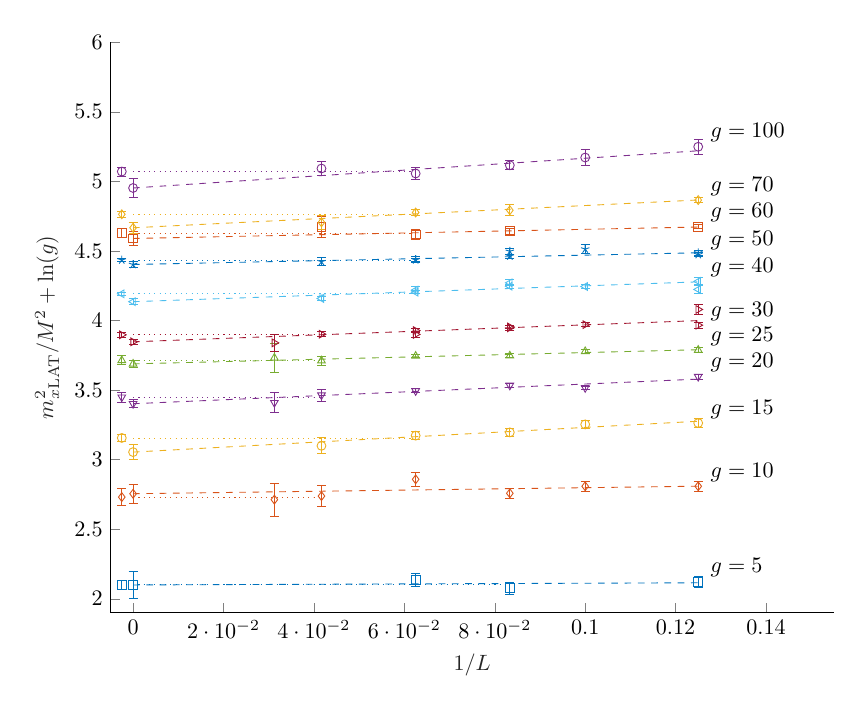
\begin{tikzpicture}[thick,scale=0.8, every node/.style={scale=1}]

\begin{axis}[%
width=4.521in,
height=3.566in,
at={(0.758in,0.481in)},
scale only axis,
xmin=-0.005,
xmax=0.155,
xlabel style={font=\color{white!15!black}},
xlabel={$1/L$},
ymin=1.9,
ymax=6,
ylabel style={font=\color{white!15!black}},
ylabel={$m_{x{\rm LAT}}^2/M^2 + \ln(g)$},
axis background/.style={fill=white},
axis x line*=bottom,
axis y line*=left
]
\addplot [color=mycolor1, dotted, forget plot]
  table[row sep=crcr]{%
0	2.10279104542099\\
0.00125	2.10279104542099\\
0.0025	2.10279104542099\\
0.00375	2.10279104542099\\
0.005	2.10279104542099\\
0.00625	2.10279104542099\\
0.0075	2.10279104542099\\
0.00875	2.10279104542099\\
0.01	2.10279104542099\\
0.01125	2.10279104542099\\
0.0125	2.10279104542099\\
0.01375	2.10279104542099\\
0.015	2.10279104542099\\
0.01625	2.10279104542099\\
0.0175	2.10279104542099\\
0.01875	2.10279104542099\\
0.02	2.10279104542099\\
0.02125	2.10279104542099\\
0.0225	2.10279104542099\\
0.02375	2.10279104542099\\
0.025	2.10279104542099\\
0.02625	2.10279104542099\\
0.0275	2.10279104542099\\
0.02875	2.10279104542099\\
0.03	2.10279104542099\\
0.03125	2.10279104542099\\
0.0325	2.10279104542099\\
0.03375	2.10279104542099\\
0.035	2.10279104542099\\
0.03625	2.10279104542099\\
0.0375	2.10279104542099\\
0.03875	2.10279104542099\\
0.04	2.10279104542099\\
0.04125	2.10279104542099\\
0.0425	2.10279104542099\\
0.04375	2.10279104542099\\
0.045	2.10279104542099\\
0.04625	2.10279104542099\\
0.0475	2.10279104542099\\
0.04875	2.10279104542099\\
0.05	2.10279104542099\\
0.05125	2.10279104542099\\
0.0525	2.10279104542099\\
0.05375	2.10279104542099\\
0.055	2.10279104542099\\
0.05625	2.10279104542099\\
0.0575	2.10279104542099\\
0.05875	2.10279104542099\\
0.06	2.10279104542099\\
0.06125	2.10279104542099\\
0.0625	2.10279104542099\\
0.06375	2.10279104542099\\
0.065	2.10279104542099\\
0.06625	2.10279104542099\\
0.0675	2.10279104542099\\
0.06875	2.10279104542099\\
0.07	2.10279104542099\\
0.07125	2.10279104542099\\
0.0725	2.10279104542099\\
0.07375	2.10279104542099\\
0.075	2.10279104542099\\
0.07625	2.10279104542099\\
0.0775	2.10279104542099\\
0.07875	2.10279104542099\\
0.08	2.10279104542099\\
0.08125	2.10279104542099\\
0.0825	2.10279104542099\\
};
\addplot [color=mycolor1, dashed, forget plot]
  table[row sep=crcr]{%
0	2.09960348442947\\
0.00125	2.09976084054418\\
0.0025	2.09991819665889\\
0.00375	2.1000755527736\\
0.005	2.10023290888831\\
0.00625	2.10039026500303\\
0.0075	2.10054762111774\\
0.00875	2.10070497723245\\
0.01	2.10086233334716\\
0.01125	2.10101968946187\\
0.0125	2.10117704557658\\
0.01375	2.10133440169129\\
0.015	2.101491757806\\
0.01625	2.10164911392072\\
0.0175	2.10180647003543\\
0.01875	2.10196382615014\\
0.02	2.10212118226485\\
0.02125	2.10227853837956\\
0.0225	2.10243589449427\\
0.02375	2.10259325060898\\
0.025	2.10275060672369\\
0.02625	2.10290796283841\\
0.0275	2.10306531895312\\
0.02875	2.10322267506783\\
0.03	2.10338003118254\\
0.03125	2.10353738729725\\
0.0325	2.10369474341196\\
0.03375	2.10385209952667\\
0.035	2.10400945564138\\
0.03625	2.10416681175609\\
0.0375	2.10432416787081\\
0.03875	2.10448152398552\\
0.04	2.10463888010023\\
0.04125	2.10479623621494\\
0.0425	2.10495359232965\\
0.04375	2.10511094844436\\
0.045	2.10526830455907\\
0.04625	2.10542566067378\\
0.0475	2.1055830167885\\
0.04875	2.10574037290321\\
0.05	2.10589772901792\\
0.05125	2.10605508513263\\
0.0525	2.10621244124734\\
0.05375	2.10636979736205\\
0.055	2.10652715347676\\
0.05625	2.10668450959147\\
0.0575	2.10684186570619\\
0.05875	2.1069992218209\\
0.06	2.10715657793561\\
0.06125	2.10731393405032\\
0.0625	2.10747129016503\\
0.06375	2.10762864627974\\
0.065	2.10778600239445\\
0.06625	2.10794335850916\\
0.0675	2.10810071462388\\
0.06875	2.10825807073859\\
0.07	2.1084154268533\\
0.07125	2.10857278296801\\
0.0725	2.10873013908272\\
0.07375	2.10888749519743\\
0.075	2.10904485131214\\
0.07625	2.10920220742685\\
0.0775	2.10935956354156\\
0.07875	2.10951691965628\\
0.08	2.10967427577099\\
0.08125	2.1098316318857\\
0.0825	2.10998898800041\\
0.08375	2.11014634411512\\
0.085	2.11030370022983\\
0.08625	2.11046105634454\\
0.0875	2.11061841245925\\
0.08875	2.11077576857397\\
0.09	2.11093312468868\\
0.09125	2.11109048080339\\
0.0925	2.1112478369181\\
0.09375	2.11140519303281\\
0.095	2.11156254914752\\
0.09625	2.11171990526223\\
0.0975	2.11187726137694\\
0.09875	2.11203461749166\\
0.1	2.11219197360637\\
0.10125	2.11234932972108\\
0.1025	2.11250668583579\\
0.10375	2.1126640419505\\
0.105	2.11282139806521\\
0.10625	2.11297875417992\\
0.1075	2.11313611029463\\
0.10875	2.11329346640935\\
0.11	2.11345082252406\\
0.11125	2.11360817863877\\
0.1125	2.11376553475348\\
0.11375	2.11392289086819\\
0.115	2.1140802469829\\
0.11625	2.11423760309761\\
0.1175	2.11439495921232\\
0.11875	2.11455231532703\\
0.12	2.11470967144175\\
0.12125	2.11486702755646\\
0.1225	2.11502438367117\\
0.12375	2.11518173978588\\
0.125	2.11533909590059\\
};
\addplot [color=mycolor1, draw=none, mark=square, mark options={solid, mycolor1}, forget plot]
 plot [error bars/.cd, y dir = both, y explicit]
 table[row sep=crcr, y error plus index=2, y error minus index=3]{%
0	2.09960348442947	0.0940854482495643	0.0940854482495643\\
-0.0025	2.10279104542099	0.032939252161526	0.032939252161526\\
0.125	2.12368661211111	0.0384201229418747	0.0384201229418747\\
0.0833333333333333	2.07692668955786	0.0442154356693399	0.0442154356693399\\
0.0625	2.13504661264345	0.0493770815069211	0.0493770815069211\\
};
\node[right, align=left]
at (axis cs:0.126,2.224) {$g = 5$};
\addplot [color=mycolor2, dotted, forget plot]
  table[row sep=crcr]{%
0	2.73119370649015\\
0.00125	2.73119370649015\\
0.0025	2.73119370649015\\
0.00375	2.73119370649015\\
0.005	2.73119370649015\\
0.00625	2.73119370649015\\
0.0075	2.73119370649015\\
0.00875	2.73119370649015\\
0.01	2.73119370649015\\
0.01125	2.73119370649015\\
0.0125	2.73119370649015\\
0.01375	2.73119370649015\\
0.015	2.73119370649015\\
0.01625	2.73119370649015\\
0.0175	2.73119370649015\\
0.01875	2.73119370649015\\
0.02	2.73119370649015\\
0.02125	2.73119370649015\\
0.0225	2.73119370649015\\
0.02375	2.73119370649015\\
0.025	2.73119370649015\\
0.02625	2.73119370649015\\
0.0275	2.73119370649015\\
0.02875	2.73119370649015\\
0.03	2.73119370649015\\
0.03125	2.73119370649015\\
0.0325	2.73119370649015\\
0.03375	2.73119370649015\\
0.035	2.73119370649015\\
0.03625	2.73119370649015\\
0.0375	2.73119370649015\\
0.03875	2.73119370649015\\
0.04	2.73119370649015\\
0.04125	2.73119370649015\\
};
\addplot [color=mycolor2, dashed, forget plot]
  table[row sep=crcr]{%
0	2.75527593509874\\
0.00125	2.75581784221291\\
0.0025	2.75635974932708\\
0.00375	2.75690165644125\\
0.005	2.75744356355542\\
0.00625	2.75798547066959\\
0.0075	2.75852737778376\\
0.00875	2.75906928489793\\
0.01	2.75961119201211\\
0.01125	2.76015309912628\\
0.0125	2.76069500624045\\
0.01375	2.76123691335462\\
0.015	2.76177882046879\\
0.01625	2.76232072758296\\
0.0175	2.76286263469713\\
0.01875	2.7634045418113\\
0.02	2.76394644892548\\
0.02125	2.76448835603965\\
0.0225	2.76503026315382\\
0.02375	2.76557217026799\\
0.025	2.76611407738216\\
0.02625	2.76665598449633\\
0.0275	2.7671978916105\\
0.02875	2.76773979872467\\
0.03	2.76828170583884\\
0.03125	2.76882361295302\\
0.0325	2.76936552006719\\
0.03375	2.76990742718136\\
0.035	2.77044933429553\\
0.03625	2.7709912414097\\
0.0375	2.77153314852387\\
0.03875	2.77207505563804\\
0.04	2.77261696275221\\
0.04125	2.77315886986639\\
0.0425	2.77370077698056\\
0.04375	2.77424268409473\\
0.045	2.7747845912089\\
0.04625	2.77532649832307\\
0.0475	2.77586840543724\\
0.04875	2.77641031255141\\
0.05	2.77695221966558\\
0.05125	2.77749412677975\\
0.0525	2.77803603389393\\
0.05375	2.7785779410081\\
0.055	2.77911984812227\\
0.05625	2.77966175523644\\
0.0575	2.78020366235061\\
0.05875	2.78074556946478\\
0.06	2.78128747657895\\
0.06125	2.78182938369312\\
0.0625	2.7823712908073\\
0.06375	2.78291319792147\\
0.065	2.78345510503564\\
0.06625	2.78399701214981\\
0.0675	2.78453891926398\\
0.06875	2.78508082637815\\
0.07	2.78562273349232\\
0.07125	2.78616464060649\\
0.0725	2.78670654772066\\
0.07375	2.78724845483484\\
0.075	2.78779036194901\\
0.07625	2.78833226906318\\
0.0775	2.78887417617735\\
0.07875	2.78941608329152\\
0.08	2.78995799040569\\
0.08125	2.79049989751986\\
0.0825	2.79104180463403\\
0.08375	2.79158371174821\\
0.085	2.79212561886238\\
0.08625	2.79266752597655\\
0.0875	2.79320943309072\\
0.08875	2.79375134020489\\
0.09	2.79429324731906\\
0.09125	2.79483515443323\\
0.0925	2.7953770615474\\
0.09375	2.79591896866157\\
0.095	2.79646087577575\\
0.09625	2.79700278288992\\
0.0975	2.79754469000409\\
0.09875	2.79808659711826\\
0.1	2.79862850423243\\
0.10125	2.7991704113466\\
0.1025	2.79971231846077\\
0.10375	2.80025422557494\\
0.105	2.80079613268912\\
0.10625	2.80133803980329\\
0.1075	2.80187994691746\\
0.10875	2.80242185403163\\
0.11	2.8029637611458\\
0.11125	2.80350566825997\\
0.1125	2.80404757537414\\
0.11375	2.80458948248831\\
0.115	2.80513138960248\\
0.11625	2.80567329671666\\
0.1175	2.80621520383083\\
0.11875	2.806757110945\\
0.12	2.80729901805917\\
0.12125	2.80784092517334\\
0.1225	2.80838283228751\\
0.12375	2.80892473940168\\
0.125	2.80946664651585\\
};
\addplot [color=mycolor2, draw=none, mark=diamond, mark options={solid, mycolor2}, forget plot]
 plot [error bars/.cd, y dir = both, y explicit]
 table[row sep=crcr, y error plus index=2, y error minus index=3]{%
0	2.75527593509874	0.0679665829360463	0.0679665829360463\\
-0.0025	2.73119370649015	0.0626053188900369	0.0626053188900369\\
0.125	2.80909615232382	0.0359980370190172	0.0359980370190172\\
0.1	2.80890117076868	0.0382287436885021	0.0382287436885021\\
0.0833333333333333	2.75829105850798	0.0369545821801482	0.0369545821801482\\
0.0625	2.85863457057082	0.0522555359080003	0.0522555359080003\\
0.0416666666666667	2.73843799740069	0.0740037317295332	0.0740037317295332\\
0.03125	2.7129591799931	0.117409415024243	0.117409415024243\\
};
\node[right, align=left]
at (axis cs:0.126,2.909) {$g = 10$};
\addplot [color=mycolor3, dotted, forget plot]
  table[row sep=crcr]{%
0	3.15612314071118\\
0.00125	3.15612314071118\\
0.0025	3.15612314071118\\
0.00375	3.15612314071118\\
0.005	3.15612314071118\\
0.00625	3.15612314071118\\
0.0075	3.15612314071118\\
0.00875	3.15612314071118\\
0.01	3.15612314071118\\
0.01125	3.15612314071118\\
0.0125	3.15612314071118\\
0.01375	3.15612314071118\\
0.015	3.15612314071118\\
0.01625	3.15612314071118\\
0.0175	3.15612314071118\\
0.01875	3.15612314071118\\
0.02	3.15612314071118\\
0.02125	3.15612314071118\\
0.0225	3.15612314071118\\
0.02375	3.15612314071118\\
0.025	3.15612314071118\\
0.02625	3.15612314071118\\
0.0275	3.15612314071118\\
0.02875	3.15612314071118\\
0.03	3.15612314071118\\
0.03125	3.15612314071118\\
0.0325	3.15612314071118\\
0.03375	3.15612314071118\\
0.035	3.15612314071118\\
0.03625	3.15612314071118\\
0.0375	3.15612314071118\\
0.03875	3.15612314071118\\
0.04	3.15612314071118\\
0.04125	3.15612314071118\\
0.0425	3.15612314071118\\
0.04375	3.15612314071118\\
0.045	3.15612314071118\\
0.04625	3.15612314071118\\
0.0475	3.15612314071118\\
0.04875	3.15612314071118\\
0.05	3.15612314071118\\
0.05125	3.15612314071118\\
0.0525	3.15612314071118\\
0.05375	3.15612314071118\\
0.055	3.15612314071118\\
0.05625	3.15612314071118\\
0.0575	3.15612314071118\\
0.05875	3.15612314071118\\
0.06	3.15612314071118\\
0.06125	3.15612314071118\\
0.0625	3.15612314071118\\
};
\addplot [color=mycolor3, dashed, forget plot]
  table[row sep=crcr]{%
0	3.05440888866837\\
0.00125	3.05662703781743\\
0.0025	3.05884518696648\\
0.00375	3.06106333611553\\
0.005	3.06328148526458\\
0.00625	3.06549963441363\\
0.0075	3.06771778356268\\
0.00875	3.06993593271174\\
0.01	3.07215408186079\\
0.01125	3.07437223100984\\
0.0125	3.07659038015889\\
0.01375	3.07880852930794\\
0.015	3.081026678457\\
0.01625	3.08324482760605\\
0.0175	3.0854629767551\\
0.01875	3.08768112590415\\
0.02	3.0898992750532\\
0.02125	3.09211742420225\\
0.0225	3.09433557335131\\
0.02375	3.09655372250036\\
0.025	3.09877187164941\\
0.02625	3.10099002079846\\
0.0275	3.10320816994751\\
0.02875	3.10542631909656\\
0.03	3.10764446824562\\
0.03125	3.10986261739467\\
0.0325	3.11208076654372\\
0.03375	3.11429891569277\\
0.035	3.11651706484182\\
0.03625	3.11873521399087\\
0.0375	3.12095336313993\\
0.03875	3.12317151228898\\
0.04	3.12538966143803\\
0.04125	3.12760781058708\\
0.0425	3.12982595973613\\
0.04375	3.13204410888518\\
0.045	3.13426225803424\\
0.04625	3.13648040718329\\
0.0475	3.13869855633234\\
0.04875	3.14091670548139\\
0.05	3.14313485463044\\
0.05125	3.1453530037795\\
0.0525	3.14757115292855\\
0.05375	3.1497893020776\\
0.055	3.15200745122665\\
0.05625	3.1542256003757\\
0.0575	3.15644374952475\\
0.05875	3.15866189867381\\
0.06	3.16088004782286\\
0.06125	3.16309819697191\\
0.0625	3.16531634612096\\
0.06375	3.16753449527001\\
0.065	3.16975264441906\\
0.06625	3.17197079356812\\
0.0675	3.17418894271717\\
0.06875	3.17640709186622\\
0.07	3.17862524101527\\
0.07125	3.18084339016432\\
0.0725	3.18306153931337\\
0.07375	3.18527968846243\\
0.075	3.18749783761148\\
0.07625	3.18971598676053\\
0.0775	3.19193413590958\\
0.07875	3.19415228505863\\
0.08	3.19637043420768\\
0.08125	3.19858858335674\\
0.0825	3.20080673250579\\
0.08375	3.20302488165484\\
0.085	3.20524303080389\\
0.08625	3.20746117995294\\
0.0875	3.20967932910199\\
0.08875	3.21189747825105\\
0.09	3.2141156274001\\
0.09125	3.21633377654915\\
0.0925	3.2185519256982\\
0.09375	3.22077007484725\\
0.095	3.22298822399631\\
0.09625	3.22520637314536\\
0.0975	3.22742452229441\\
0.09875	3.22964267144346\\
0.1	3.23186082059251\\
0.10125	3.23407896974156\\
0.1025	3.23629711889062\\
0.10375	3.23851526803967\\
0.105	3.24073341718872\\
0.10625	3.24295156633777\\
0.1075	3.24516971548682\\
0.10875	3.24738786463587\\
0.11	3.24960601378493\\
0.11125	3.25182416293398\\
0.1125	3.25404231208303\\
0.11375	3.25626046123208\\
0.115	3.25847861038113\\
0.11625	3.26069675953018\\
0.1175	3.26291490867924\\
0.11875	3.26513305782829\\
0.12	3.26735120697734\\
0.12125	3.26956935612639\\
0.1225	3.27178750527544\\
0.12375	3.27400565442449\\
0.125	3.27622380357355\\
};
\addplot [color=mycolor3, draw=none, mark=o, mark options={solid, mycolor3}, forget plot]
 plot [error bars/.cd, y dir = both, y explicit]
 table[row sep=crcr, y error plus index=2, y error minus index=3]{%
0	3.05440888866837	0.0532360302975794	0.0532360302975794\\
-0.0025	3.15612314071118	0.0270631585014332	0.0270631585014332\\
0.125	3.2631599869947	0.0301167596084888	0.0301167596084888\\
0.1	3.2535476598451	0.0304080795714759	0.0304080795714759\\
0.0833333333333333	3.19617831842811	0.0277179558752633	0.0277179558752633\\
0.0625	3.17274214064008	0.0307782633721614	0.0307782633721614\\
0.0416666666666667	3.0994794151236	0.0568221384166933	0.0568221384166933\\
};
\node[right, align=left]
at (axis cs:0.126,3.363) {$g = 15$};
\addplot [color=mycolor4, dotted, forget plot]
  table[row sep=crcr]{%
0	3.44910679512875\\
0.00125	3.44910679512875\\
0.0025	3.44910679512875\\
0.00375	3.44910679512875\\
0.005	3.44910679512875\\
0.00625	3.44910679512875\\
0.0075	3.44910679512875\\
0.00875	3.44910679512875\\
0.01	3.44910679512875\\
0.01125	3.44910679512875\\
0.0125	3.44910679512875\\
0.01375	3.44910679512875\\
0.015	3.44910679512875\\
0.01625	3.44910679512875\\
0.0175	3.44910679512875\\
0.01875	3.44910679512875\\
0.02	3.44910679512875\\
0.02125	3.44910679512875\\
0.0225	3.44910679512875\\
0.02375	3.44910679512875\\
0.025	3.44910679512875\\
0.02625	3.44910679512875\\
0.0275	3.44910679512875\\
0.02875	3.44910679512875\\
0.03	3.44910679512875\\
0.03125	3.44910679512875\\
0.0325	3.44910679512875\\
0.03375	3.44910679512875\\
0.035	3.44910679512875\\
0.03625	3.44910679512875\\
0.0375	3.44910679512875\\
0.03875	3.44910679512875\\
0.04	3.44910679512875\\
0.04125	3.44910679512875\\
};
\addplot [color=mycolor4, dashed, forget plot]
  table[row sep=crcr]{%
0	3.4019951488216\\
0.00125	3.40376454431439\\
0.0025	3.40553393980719\\
0.00375	3.40730333529999\\
0.005	3.40907273079278\\
0.00625	3.41084212628558\\
0.0075	3.41261152177838\\
0.00875	3.41438091727118\\
0.01	3.41615031276397\\
0.01125	3.41791970825677\\
0.0125	3.41968910374957\\
0.01375	3.42145849924236\\
0.015	3.42322789473516\\
0.01625	3.42499729022796\\
0.0175	3.42676668572076\\
0.01875	3.42853608121355\\
0.02	3.43030547670635\\
0.02125	3.43207487219915\\
0.0225	3.43384426769194\\
0.02375	3.43561366318474\\
0.025	3.43738305867754\\
0.02625	3.43915245417034\\
0.0275	3.44092184966313\\
0.02875	3.44269124515593\\
0.03	3.44446064064873\\
0.03125	3.44623003614152\\
0.0325	3.44799943163432\\
0.03375	3.44976882712712\\
0.035	3.45153822261992\\
0.03625	3.45330761811271\\
0.0375	3.45507701360551\\
0.03875	3.45684640909831\\
0.04	3.4586158045911\\
0.04125	3.4603852000839\\
0.0425	3.4621545955767\\
0.04375	3.4639239910695\\
0.045	3.46569338656229\\
0.04625	3.46746278205509\\
0.0475	3.46923217754789\\
0.04875	3.47100157304068\\
0.05	3.47277096853348\\
0.05125	3.47454036402628\\
0.0525	3.47630975951908\\
0.05375	3.47807915501187\\
0.055	3.47984855050467\\
0.05625	3.48161794599747\\
0.0575	3.48338734149026\\
0.05875	3.48515673698306\\
0.06	3.48692613247586\\
0.06125	3.48869552796866\\
0.0625	3.49046492346145\\
0.06375	3.49223431895425\\
0.065	3.49400371444705\\
0.06625	3.49577310993984\\
0.0675	3.49754250543264\\
0.06875	3.49931190092544\\
0.07	3.50108129641824\\
0.07125	3.50285069191103\\
0.0725	3.50462008740383\\
0.07375	3.50638948289663\\
0.075	3.50815887838942\\
0.07625	3.50992827388222\\
0.0775	3.51169766937502\\
0.07875	3.51346706486782\\
0.08	3.51523646036061\\
0.08125	3.51700585585341\\
0.0825	3.51877525134621\\
0.08375	3.520544646839\\
0.085	3.5223140423318\\
0.08625	3.5240834378246\\
0.0875	3.5258528333174\\
0.08875	3.52762222881019\\
0.09	3.52939162430299\\
0.09125	3.53116101979579\\
0.0925	3.53293041528858\\
0.09375	3.53469981078138\\
0.095	3.53646920627418\\
0.09625	3.53823860176698\\
0.0975	3.54000799725977\\
0.09875	3.54177739275257\\
0.1	3.54354678824537\\
0.10125	3.54531618373816\\
0.1025	3.54708557923096\\
0.10375	3.54885497472376\\
0.105	3.55062437021656\\
0.10625	3.55239376570935\\
0.1075	3.55416316120215\\
0.10875	3.55593255669495\\
0.11	3.55770195218774\\
0.11125	3.55947134768054\\
0.1125	3.56124074317334\\
0.11375	3.56301013866614\\
0.115	3.56477953415893\\
0.11625	3.56654892965173\\
0.1175	3.56831832514453\\
0.11875	3.57008772063732\\
0.12	3.57185711613012\\
0.12125	3.57362651162292\\
0.1225	3.57539590711572\\
0.12375	3.57716530260851\\
0.125	3.57893469810131\\
};
\addplot [color=mycolor4, draw=none, mark=triangle, mark options={solid, rotate=180, mycolor4}, forget plot]
 plot [error bars/.cd, y dir = both, y explicit]
 table[row sep=crcr, y error plus index=2, y error minus index=3]{%
0	3.4019951488216	0.0281024418118495	0.0281024418118495\\
-0.0025	3.44910679512875	0.0369182826303483	0.0369182826303483\\
0.125	3.59656065569458	0.0168479399073513	0.0168479399073513\\
0.1	3.51628704764306	0.013348009674409	0.013348009674409\\
0.0833333333333333	3.53381050421518	0.0131851587445629	0.0131851587445629\\
0.0625	3.49404518837739	0.0145236442693891	0.0145236442693891\\
0.0416666666666667	3.46381479881602	0.0432576734950238	0.0432576734950238\\
0.03125	3.40966605708617	0.0708367797442081	0.0708367797442081\\
};
\node[right, align=left]
at (axis cs:0.126,3.697) {$g = 20$};
\addplot [color=mycolor5, dotted, forget plot]
  table[row sep=crcr]{%
0	3.71347727627448\\
0.00125	3.71347727627448\\
0.0025	3.71347727627448\\
0.00375	3.71347727627448\\
0.005	3.71347727627448\\
0.00625	3.71347727627448\\
0.0075	3.71347727627448\\
0.00875	3.71347727627448\\
0.01	3.71347727627448\\
0.01125	3.71347727627448\\
0.0125	3.71347727627448\\
0.01375	3.71347727627448\\
0.015	3.71347727627448\\
0.01625	3.71347727627448\\
0.0175	3.71347727627448\\
0.01875	3.71347727627448\\
0.02	3.71347727627448\\
0.02125	3.71347727627448\\
0.0225	3.71347727627448\\
0.02375	3.71347727627448\\
0.025	3.71347727627448\\
0.02625	3.71347727627448\\
0.0275	3.71347727627448\\
0.02875	3.71347727627448\\
0.03	3.71347727627448\\
0.03125	3.71347727627448\\
0.0325	3.71347727627448\\
0.03375	3.71347727627448\\
0.035	3.71347727627448\\
0.03625	3.71347727627448\\
0.0375	3.71347727627448\\
0.03875	3.71347727627448\\
0.04	3.71347727627448\\
0.04125	3.71347727627448\\
};
\addplot [color=mycolor5, dashed, forget plot]
  table[row sep=crcr]{%
0	3.68831307892431\\
0.00125	3.68932992539674\\
0.0025	3.69034677186916\\
0.00375	3.69136361834158\\
0.005	3.692380464814\\
0.00625	3.69339731128642\\
0.0075	3.69441415775884\\
0.00875	3.69543100423126\\
0.01	3.69644785070369\\
0.01125	3.69746469717611\\
0.0125	3.69848154364853\\
0.01375	3.69949839012095\\
0.015	3.70051523659337\\
0.01625	3.70153208306579\\
0.0175	3.70254892953822\\
0.01875	3.70356577601064\\
0.02	3.70458262248306\\
0.02125	3.70559946895548\\
0.0225	3.7066163154279\\
0.02375	3.70763316190033\\
0.025	3.70865000837275\\
0.02625	3.70966685484517\\
0.0275	3.71068370131759\\
0.02875	3.71170054779001\\
0.03	3.71271739426243\\
0.03125	3.71373424073486\\
0.0325	3.71475108720728\\
0.03375	3.7157679336797\\
0.035	3.71678478015212\\
0.03625	3.71780162662454\\
0.0375	3.71881847309696\\
0.03875	3.71983531956939\\
0.04	3.72085216604181\\
0.04125	3.72186901251423\\
0.0425	3.72288585898665\\
0.04375	3.72390270545907\\
0.045	3.72491955193149\\
0.04625	3.72593639840392\\
0.0475	3.72695324487634\\
0.04875	3.72797009134876\\
0.05	3.72898693782118\\
0.05125	3.7300037842936\\
0.0525	3.73102063076602\\
0.05375	3.73203747723845\\
0.055	3.73305432371087\\
0.05625	3.73407117018329\\
0.0575	3.73508801665571\\
0.05875	3.73610486312813\\
0.06	3.73712170960055\\
0.06125	3.73813855607298\\
0.0625	3.7391554025454\\
0.06375	3.74017224901782\\
0.065	3.74118909549024\\
0.06625	3.74220594196266\\
0.0675	3.74322278843508\\
0.06875	3.74423963490751\\
0.07	3.74525648137993\\
0.07125	3.74627332785235\\
0.0725	3.74729017432477\\
0.07375	3.74830702079719\\
0.075	3.74932386726961\\
0.07625	3.75034071374204\\
0.0775	3.75135756021446\\
0.07875	3.75237440668688\\
0.08	3.7533912531593\\
0.08125	3.75440809963172\\
0.0825	3.75542494610414\\
0.08375	3.75644179257657\\
0.085	3.75745863904899\\
0.08625	3.75847548552141\\
0.0875	3.75949233199383\\
0.08875	3.76050917846625\\
0.09	3.76152602493867\\
0.09125	3.7625428714111\\
0.0925	3.76355971788352\\
0.09375	3.76457656435594\\
0.095	3.76559341082836\\
0.09625	3.76661025730078\\
0.0975	3.7676271037732\\
0.09875	3.76864395024563\\
0.1	3.76966079671805\\
0.10125	3.77067764319047\\
0.1025	3.77169448966289\\
0.10375	3.77271133613531\\
0.105	3.77372818260773\\
0.10625	3.77474502908016\\
0.1075	3.77576187555258\\
0.10875	3.776778722025\\
0.11	3.77779556849742\\
0.11125	3.77881241496984\\
0.1125	3.77982926144226\\
0.11375	3.78084610791469\\
0.115	3.78186295438711\\
0.11625	3.78287980085953\\
0.1175	3.78389664733195\\
0.11875	3.78491349380437\\
0.12	3.78593034027679\\
0.12125	3.78694718674922\\
0.1225	3.78796403322164\\
0.12375	3.78898087969406\\
0.125	3.78999772616648\\
};
\addplot [color=mycolor5, draw=none, mark=triangle, mark options={solid, mycolor5}, forget plot]
 plot [error bars/.cd, y dir = both, y explicit]
 table[row sep=crcr, y error plus index=2, y error minus index=3]{%
0	3.68831307892431	0.0268544852814218	0.0268544852814218\\
-0.0025	3.71347727627448	0.0320155698372206	0.0320155698372206\\
0.125	3.78765923731392	0.0172809633867572	0.0172809633867572\\
0.1	3.77797904147837	0.0144514065818716	0.0144514065818716\\
0.0833333333333333	3.74674927329836	0.0130363188094429	0.0130363188094429\\
0.0625	3.74476573810957	0.0135112786187543	0.0135112786187543\\
0.0416666666666667	3.71149795455967	0.0337425795570016	0.0337425795570016\\
0.03125	3.73134192566314	0.101371841174389	0.101371841174389\\
};
\node[right, align=left]
at (axis cs:0.126,3.888) {$g = 25$};
\addplot [color=mycolor6, dotted, forget plot]
  table[row sep=crcr]{%
0	3.89706098090586\\
0.00125	3.89706098090586\\
0.0025	3.89706098090586\\
0.00375	3.89706098090586\\
0.005	3.89706098090586\\
0.00625	3.89706098090586\\
0.0075	3.89706098090586\\
0.00875	3.89706098090586\\
0.01	3.89706098090586\\
0.01125	3.89706098090586\\
0.0125	3.89706098090586\\
0.01375	3.89706098090586\\
0.015	3.89706098090586\\
0.01625	3.89706098090586\\
0.0175	3.89706098090586\\
0.01875	3.89706098090586\\
0.02	3.89706098090586\\
0.02125	3.89706098090586\\
0.0225	3.89706098090586\\
0.02375	3.89706098090586\\
0.025	3.89706098090586\\
0.02625	3.89706098090586\\
0.0275	3.89706098090586\\
0.02875	3.89706098090586\\
0.03	3.89706098090586\\
0.03125	3.89706098090586\\
0.0325	3.89706098090586\\
0.03375	3.89706098090586\\
0.035	3.89706098090586\\
0.03625	3.89706098090586\\
0.0375	3.89706098090586\\
0.03875	3.89706098090586\\
0.04	3.89706098090586\\
0.04125	3.89706098090586\\
};
\addplot [color=mycolor6, dashed, forget plot]
  table[row sep=crcr]{%
0	3.84694860448127\\
0.00125	3.84847264275297\\
0.0025	3.84999668102468\\
0.00375	3.85152071929638\\
0.005	3.85304475756808\\
0.00625	3.85456879583978\\
0.0075	3.85609283411149\\
0.00875	3.85761687238319\\
0.01	3.85914091065489\\
0.01125	3.86066494892659\\
0.0125	3.86218898719829\\
0.01375	3.86371302547\\
0.015	3.8652370637417\\
0.01625	3.8667611020134\\
0.0175	3.8682851402851\\
0.01875	3.8698091785568\\
0.02	3.87133321682851\\
0.02125	3.87285725510021\\
0.0225	3.87438129337191\\
0.02375	3.87590533164361\\
0.025	3.87742936991532\\
0.02625	3.87895340818702\\
0.0275	3.88047744645872\\
0.02875	3.88200148473042\\
0.03	3.88352552300212\\
0.03125	3.88504956127383\\
0.0325	3.88657359954553\\
0.03375	3.88809763781723\\
0.035	3.88962167608893\\
0.03625	3.89114571436064\\
0.0375	3.89266975263234\\
0.03875	3.89419379090404\\
0.04	3.89571782917574\\
0.04125	3.89724186744744\\
0.0425	3.89876590571915\\
0.04375	3.90028994399085\\
0.045	3.90181398226255\\
0.04625	3.90333802053425\\
0.0475	3.90486205880596\\
0.04875	3.90638609707766\\
0.05	3.90791013534936\\
0.05125	3.90943417362106\\
0.0525	3.91095821189276\\
0.05375	3.91248225016447\\
0.055	3.91400628843617\\
0.05625	3.91553032670787\\
0.0575	3.91705436497957\\
0.05875	3.91857840325128\\
0.06	3.92010244152298\\
0.06125	3.92162647979468\\
0.0625	3.92315051806638\\
0.06375	3.92467455633808\\
0.065	3.92619859460979\\
0.06625	3.92772263288149\\
0.0675	3.92924667115319\\
0.06875	3.93077070942489\\
0.07	3.9322947476966\\
0.07125	3.9338187859683\\
0.0725	3.93534282424\\
0.07375	3.9368668625117\\
0.075	3.9383909007834\\
0.07625	3.93991493905511\\
0.0775	3.94143897732681\\
0.07875	3.94296301559851\\
0.08	3.94448705387021\\
0.08125	3.94601109214191\\
0.0825	3.94753513041362\\
0.08375	3.94905916868532\\
0.085	3.95058320695702\\
0.08625	3.95210724522872\\
0.0875	3.95363128350043\\
0.08875	3.95515532177213\\
0.09	3.95667936004383\\
0.09125	3.95820339831553\\
0.0925	3.95972743658723\\
0.09375	3.96125147485894\\
0.095	3.96277551313064\\
0.09625	3.96429955140234\\
0.0975	3.96582358967404\\
0.09875	3.96734762794575\\
0.1	3.96887166621745\\
0.10125	3.97039570448915\\
0.1025	3.97191974276085\\
0.10375	3.97344378103255\\
0.105	3.97496781930426\\
0.10625	3.97649185757596\\
0.1075	3.97801589584766\\
0.10875	3.97953993411936\\
0.11	3.98106397239106\\
0.11125	3.98258801066277\\
0.1125	3.98411204893447\\
0.11375	3.98563608720617\\
0.115	3.98716012547787\\
0.11625	3.98868416374958\\
0.1175	3.99020820202128\\
0.11875	3.99173224029298\\
0.12	3.99325627856468\\
0.12125	3.99478031683638\\
0.1225	3.99630435510809\\
0.12375	3.99782839337979\\
0.125	3.99935243165149\\
};
\addplot [color=mycolor6, draw=none, mark=triangle, mark options={solid, rotate=270, mycolor6}, forget plot]
 plot [error bars/.cd, y dir = both, y explicit]
 table[row sep=crcr, y error plus index=2, y error minus index=3]{%
0	3.84694860448127	0.0201282079389417	0.0201282079389417\\
-0.0025	3.89706098090586	0.0158242715593936	0.0158242715593936\\
0.125	3.9665558733127	0.0199852026768696	0.0199852026768696\\
0.1	3.97033969690974	0.0144883556381705	0.0144883556381705\\
0.0833333333333333	3.95391736211314	0.0137349248582794	0.0137349248582794\\
0.0625	3.92739445063454	0.0134919399658943	0.0134919399658943\\
0.0416666666666667	3.90155588295543	0.0164291954544859	0.0164291954544859\\
0.03125	3.83937230887339	0.0588574511876925	0.0588574511876925\\
0.125	4.07933663826855	0.0345470273676876	0.0345470273676876\\
0.0833333333333333	3.94804817275862	0.0187999867095485	0.0187999867095485\\
0.0625	3.90037379286465	0.0229752431514439	0.0229752431514439\\
};
\node[right, align=left]
at (axis cs:0.126,4.067) {$g = 30$};
\addplot [color=mycolor7, dotted, forget plot]
  table[row sep=crcr]{%
0	4.19172788147305\\
0.00125	4.19172788147305\\
0.0025	4.19172788147305\\
0.00375	4.19172788147305\\
0.005	4.19172788147305\\
0.00625	4.19172788147305\\
0.0075	4.19172788147305\\
0.00875	4.19172788147305\\
0.01	4.19172788147305\\
0.01125	4.19172788147305\\
0.0125	4.19172788147305\\
0.01375	4.19172788147305\\
0.015	4.19172788147305\\
0.01625	4.19172788147305\\
0.0175	4.19172788147305\\
0.01875	4.19172788147305\\
0.02	4.19172788147305\\
0.02125	4.19172788147305\\
0.0225	4.19172788147305\\
0.02375	4.19172788147305\\
0.025	4.19172788147305\\
0.02625	4.19172788147305\\
0.0275	4.19172788147305\\
0.02875	4.19172788147305\\
0.03	4.19172788147305\\
0.03125	4.19172788147305\\
0.0325	4.19172788147305\\
0.03375	4.19172788147305\\
0.035	4.19172788147305\\
0.03625	4.19172788147305\\
0.0375	4.19172788147305\\
0.03875	4.19172788147305\\
0.04	4.19172788147305\\
0.04125	4.19172788147305\\
0.0425	4.19172788147305\\
0.04375	4.19172788147305\\
0.045	4.19172788147305\\
0.04625	4.19172788147305\\
0.0475	4.19172788147305\\
0.04875	4.19172788147305\\
0.05	4.19172788147305\\
0.05125	4.19172788147305\\
0.0525	4.19172788147305\\
0.05375	4.19172788147305\\
0.055	4.19172788147305\\
0.05625	4.19172788147305\\
0.0575	4.19172788147305\\
0.05875	4.19172788147305\\
0.06	4.19172788147305\\
0.06125	4.19172788147305\\
0.0625	4.19172788147305\\
};
\addplot [color=mycolor7, dashed, forget plot]
  table[row sep=crcr]{%
0	4.1351993565938\\
0.00125	4.13662369650335\\
0.0025	4.1380480364129\\
0.00375	4.13947237632245\\
0.005	4.140896716232\\
0.00625	4.14232105614156\\
0.0075	4.14374539605111\\
0.00875	4.14516973596066\\
0.01	4.14659407587021\\
0.01125	4.14801841577976\\
0.0125	4.14944275568931\\
0.01375	4.15086709559887\\
0.015	4.15229143550842\\
0.01625	4.15371577541797\\
0.0175	4.15514011532752\\
0.01875	4.15656445523707\\
0.02	4.15798879514662\\
0.02125	4.15941313505618\\
0.0225	4.16083747496573\\
0.02375	4.16226181487528\\
0.025	4.16368615478483\\
0.02625	4.16511049469438\\
0.0275	4.16653483460393\\
0.02875	4.16795917451349\\
0.03	4.16938351442304\\
0.03125	4.17080785433259\\
0.0325	4.17223219424214\\
0.03375	4.17365653415169\\
0.035	4.17508087406124\\
0.03625	4.1765052139708\\
0.0375	4.17792955388035\\
0.03875	4.1793538937899\\
0.04	4.18077823369945\\
0.04125	4.182202573609\\
0.0425	4.18362691351855\\
0.04375	4.18505125342811\\
0.045	4.18647559333766\\
0.04625	4.18789993324721\\
0.0475	4.18932427315676\\
0.04875	4.19074861306631\\
0.05	4.19217295297586\\
0.05125	4.19359729288542\\
0.0525	4.19502163279497\\
0.05375	4.19644597270452\\
0.055	4.19787031261407\\
0.05625	4.19929465252362\\
0.0575	4.20071899243317\\
0.05875	4.20214333234273\\
0.06	4.20356767225228\\
0.06125	4.20499201216183\\
0.0625	4.20641635207138\\
0.06375	4.20784069198093\\
0.065	4.20926503189048\\
0.06625	4.21068937180004\\
0.0675	4.21211371170959\\
0.06875	4.21353805161914\\
0.07	4.21496239152869\\
0.07125	4.21638673143824\\
0.0725	4.21781107134779\\
0.07375	4.21923541125735\\
0.075	4.2206597511669\\
0.07625	4.22208409107645\\
0.0775	4.223508430986\\
0.07875	4.22493277089555\\
0.08	4.2263571108051\\
0.08125	4.22778145071466\\
0.0825	4.22920579062421\\
0.08375	4.23063013053376\\
0.085	4.23205447044331\\
0.08625	4.23347881035286\\
0.0875	4.23490315026241\\
0.08875	4.23632749017197\\
0.09	4.23775183008152\\
0.09125	4.23917616999107\\
0.0925	4.24060050990062\\
0.09375	4.24202484981017\\
0.095	4.24344918971972\\
0.09625	4.24487352962928\\
0.0975	4.24629786953883\\
0.09875	4.24772220944838\\
0.1	4.24914654935793\\
0.10125	4.25057088926748\\
0.1025	4.25199522917703\\
0.10375	4.25341956908659\\
0.105	4.25484390899614\\
0.10625	4.25626824890569\\
0.1075	4.25769258881524\\
0.10875	4.25911692872479\\
0.11	4.26054126863434\\
0.11125	4.2619656085439\\
0.1125	4.26338994845345\\
0.11375	4.264814288363\\
0.115	4.26623862827255\\
0.11625	4.2676629681821\\
0.1175	4.26908730809165\\
0.11875	4.27051164800121\\
0.12	4.27193598791076\\
0.12125	4.27336032782031\\
0.1225	4.27478466772986\\
0.12375	4.27620900763941\\
0.125	4.27763334754896\\
};
\addplot [color=mycolor7, draw=none, mark=triangle, mark options={solid, rotate=90, mycolor7}, forget plot]
 plot [error bars/.cd, y dir = both, y explicit]
 table[row sep=crcr, y error plus index=2, y error minus index=3]{%
0	4.1351993565938	0.0213564289850636	0.0213564289850636\\
-0.0025	4.19172788147305	0.00955250259884957	0.00955250259884957\\
0.125	4.28122152200913	0.0250201618105598	0.0250201618105598\\
0.1	4.244201780252	0.0158414605231274	0.0158414605231274\\
0.0833333333333333	4.24607906079525	0.0138240682772275	0.0138240682772275\\
0.0625	4.20375925091581	0.0126014703491007	0.0126014703491007\\
0.0416666666666667	4.15808029616339	0.0173710197367235	0.0173710197367235\\
0.125	4.2232092014991	0.0261223810508101	0.0261223810508101\\
0.0833333333333333	4.27068039249291	0.0209081368371978	0.0209081368371978\\
0.0625	4.21825136710321	0.0272413307701072	0.0272413307701072\\
};
\node[right, align=left]
at (axis cs:0.126,4.381) {$g = 40$};
\addplot [color=mycolor1, dotted, forget plot]
  table[row sep=crcr]{%
0	4.43468324199569\\
0.00125	4.43468324199569\\
0.0025	4.43468324199569\\
0.00375	4.43468324199569\\
0.005	4.43468324199569\\
0.00625	4.43468324199569\\
0.0075	4.43468324199569\\
0.00875	4.43468324199569\\
0.01	4.43468324199569\\
0.01125	4.43468324199569\\
0.0125	4.43468324199569\\
0.01375	4.43468324199569\\
0.015	4.43468324199569\\
0.01625	4.43468324199569\\
0.0175	4.43468324199569\\
0.01875	4.43468324199569\\
0.02	4.43468324199569\\
0.02125	4.43468324199569\\
0.0225	4.43468324199569\\
0.02375	4.43468324199569\\
0.025	4.43468324199569\\
0.02625	4.43468324199569\\
0.0275	4.43468324199569\\
0.02875	4.43468324199569\\
0.03	4.43468324199569\\
0.03125	4.43468324199569\\
0.0325	4.43468324199569\\
0.03375	4.43468324199569\\
0.035	4.43468324199569\\
0.03625	4.43468324199569\\
0.0375	4.43468324199569\\
0.03875	4.43468324199569\\
0.04	4.43468324199569\\
0.04125	4.43468324199569\\
0.0425	4.43468324199569\\
0.04375	4.43468324199569\\
0.045	4.43468324199569\\
0.04625	4.43468324199569\\
0.0475	4.43468324199569\\
0.04875	4.43468324199569\\
0.05	4.43468324199569\\
0.05125	4.43468324199569\\
0.0525	4.43468324199569\\
0.05375	4.43468324199569\\
0.055	4.43468324199569\\
0.05625	4.43468324199569\\
0.0575	4.43468324199569\\
0.05875	4.43468324199569\\
0.06	4.43468324199569\\
0.06125	4.43468324199569\\
0.0625	4.43468324199569\\
};
\addplot [color=mycolor1, dashed, forget plot]
  table[row sep=crcr]{%
0	4.40250943478156\\
0.00125	4.40335020465921\\
0.0025	4.40419097453687\\
0.00375	4.40503174441453\\
0.005	4.40587251429218\\
0.00625	4.40671328416984\\
0.0075	4.40755405404749\\
0.00875	4.40839482392515\\
0.01	4.40923559380281\\
0.01125	4.41007636368046\\
0.0125	4.41091713355812\\
0.01375	4.41175790343578\\
0.015	4.41259867331343\\
0.01625	4.41343944319109\\
0.0175	4.41428021306875\\
0.01875	4.4151209829464\\
0.02	4.41596175282406\\
0.02125	4.41680252270172\\
0.0225	4.41764329257937\\
0.02375	4.41848406245703\\
0.025	4.41932483233469\\
0.02625	4.42016560221234\\
0.0275	4.42100637209\\
0.02875	4.42184714196766\\
0.03	4.42268791184531\\
0.03125	4.42352868172297\\
0.0325	4.42436945160062\\
0.03375	4.42521022147828\\
0.035	4.42605099135594\\
0.03625	4.42689176123359\\
0.0375	4.42773253111125\\
0.03875	4.42857330098891\\
0.04	4.42941407086656\\
0.04125	4.43025484074422\\
0.0425	4.43109561062188\\
0.04375	4.43193638049953\\
0.045	4.43277715037719\\
0.04625	4.43361792025485\\
0.0475	4.4344586901325\\
0.04875	4.43529946001016\\
0.05	4.43614022988781\\
0.05125	4.43698099976547\\
0.0525	4.43782176964313\\
0.05375	4.43866253952078\\
0.055	4.43950330939844\\
0.05625	4.4403440792761\\
0.0575	4.44118484915375\\
0.05875	4.44202561903141\\
0.06	4.44286638890907\\
0.06125	4.44370715878672\\
0.0625	4.44454792866438\\
0.06375	4.44538869854204\\
0.065	4.44622946841969\\
0.06625	4.44707023829735\\
0.0675	4.44791100817501\\
0.06875	4.44875177805266\\
0.07	4.44959254793032\\
0.07125	4.45043331780797\\
0.0725	4.45127408768563\\
0.07375	4.45211485756329\\
0.075	4.45295562744094\\
0.07625	4.4537963973186\\
0.0775	4.45463716719626\\
0.07875	4.45547793707391\\
0.08	4.45631870695157\\
0.08125	4.45715947682923\\
0.0825	4.45800024670688\\
0.08375	4.45884101658454\\
0.085	4.4596817864622\\
0.08625	4.46052255633985\\
0.0875	4.46136332621751\\
0.08875	4.46220409609517\\
0.09	4.46304486597282\\
0.09125	4.46388563585048\\
0.0925	4.46472640572813\\
0.09375	4.46556717560579\\
0.095	4.46640794548345\\
0.09625	4.4672487153611\\
0.0975	4.46808948523876\\
0.09875	4.46893025511642\\
0.1	4.46977102499407\\
0.10125	4.47061179487173\\
0.1025	4.47145256474939\\
0.10375	4.47229333462704\\
0.105	4.4731341045047\\
0.10625	4.47397487438236\\
0.1075	4.47481564426001\\
0.10875	4.47565641413767\\
0.11	4.47649718401532\\
0.11125	4.47733795389298\\
0.1125	4.47817872377064\\
0.11375	4.47901949364829\\
0.115	4.47986026352595\\
0.11625	4.48070103340361\\
0.1175	4.48154180328126\\
0.11875	4.48238257315892\\
0.12	4.48322334303658\\
0.12125	4.48406411291423\\
0.1225	4.48490488279189\\
0.12375	4.48574565266955\\
0.125	4.4865864225472\\
};
\addplot [color=mycolor1, draw=none, mark=star, mark options={solid, mycolor1}, forget plot]
 plot [error bars/.cd, y dir = both, y explicit]
 table[row sep=crcr, y error plus index=2, y error minus index=3]{%
0	4.40250943478156	0.0206704061178771	0.0206704061178771\\
-0.0025	4.43468324199569	0.00969387710895657	0.00969387710895657\\
0.125	4.47338943250936	0.0143270859465311	0.0143270859465311\\
0.1	4.51334030181675	0.032385530467198	0.032385530467198\\
0.0833333333333333	4.46309731467542	0.013908832325894	0.013908832325894\\
0.0625	4.4359934339765	0.0114649528843551	0.0114649528843551\\
0.0416666666666667	4.42260979716466	0.0280066011284326	0.0280066011284326\\
0.125	4.48620373908551	0.0202700263256076	0.0202700263256076\\
0.0833333333333333	4.49726975517878	0.0210519321773921	0.0210519321773921\\
0.0625	4.43776751460988	0.0238439703651342	0.0238439703651342\\
};
\node[right, align=left]
at (axis cs:0.126,4.573) {$g = 50$};
\addplot [color=mycolor2, dotted, forget plot]
  table[row sep=crcr]{%
0	4.62854217784568\\
0.00125	4.62854217784568\\
0.0025	4.62854217784568\\
0.00375	4.62854217784568\\
0.005	4.62854217784568\\
0.00625	4.62854217784568\\
0.0075	4.62854217784568\\
0.00875	4.62854217784568\\
0.01	4.62854217784568\\
0.01125	4.62854217784568\\
0.0125	4.62854217784568\\
0.01375	4.62854217784568\\
0.015	4.62854217784568\\
0.01625	4.62854217784568\\
0.0175	4.62854217784568\\
0.01875	4.62854217784568\\
0.02	4.62854217784568\\
0.02125	4.62854217784568\\
0.0225	4.62854217784568\\
0.02375	4.62854217784568\\
0.025	4.62854217784568\\
0.02625	4.62854217784568\\
0.0275	4.62854217784568\\
0.02875	4.62854217784568\\
0.03	4.62854217784568\\
0.03125	4.62854217784568\\
0.0325	4.62854217784568\\
0.03375	4.62854217784568\\
0.035	4.62854217784568\\
0.03625	4.62854217784568\\
0.0375	4.62854217784568\\
0.03875	4.62854217784568\\
0.04	4.62854217784568\\
0.04125	4.62854217784568\\
0.0425	4.62854217784568\\
0.04375	4.62854217784568\\
0.045	4.62854217784568\\
0.04625	4.62854217784568\\
0.0475	4.62854217784568\\
0.04875	4.62854217784568\\
0.05	4.62854217784568\\
0.05125	4.62854217784568\\
0.0525	4.62854217784568\\
0.05375	4.62854217784568\\
0.055	4.62854217784568\\
0.05625	4.62854217784568\\
0.0575	4.62854217784568\\
0.05875	4.62854217784568\\
0.06	4.62854217784568\\
0.06125	4.62854217784568\\
0.0625	4.62854217784568\\
};
\addplot [color=mycolor2, dashed, forget plot]
  table[row sep=crcr]{%
0	4.58945203344531\\
0.00125	4.59027490190877\\
0.0025	4.59109777037222\\
0.00375	4.59192063883567\\
0.005	4.59274350729912\\
0.00625	4.59356637576257\\
0.0075	4.59438924422602\\
0.00875	4.59521211268947\\
0.01	4.59603498115292\\
0.01125	4.59685784961638\\
0.0125	4.59768071807983\\
0.01375	4.59850358654328\\
0.015	4.59932645500673\\
0.01625	4.60014932347018\\
0.0175	4.60097219193363\\
0.01875	4.60179506039708\\
0.02	4.60261792886053\\
0.02125	4.60344079732399\\
0.0225	4.60426366578744\\
0.02375	4.60508653425089\\
0.025	4.60590940271434\\
0.02625	4.60673227117779\\
0.0275	4.60755513964124\\
0.02875	4.60837800810469\\
0.03	4.60920087656814\\
0.03125	4.6100237450316\\
0.0325	4.61084661349505\\
0.03375	4.6116694819585\\
0.035	4.61249235042195\\
0.03625	4.6133152188854\\
0.0375	4.61413808734885\\
0.03875	4.6149609558123\\
0.04	4.61578382427575\\
0.04125	4.61660669273921\\
0.0425	4.61742956120266\\
0.04375	4.61825242966611\\
0.045	4.61907529812956\\
0.04625	4.61989816659301\\
0.0475	4.62072103505646\\
0.04875	4.62154390351991\\
0.05	4.62236677198336\\
0.05125	4.62318964044682\\
0.0525	4.62401250891027\\
0.05375	4.62483537737372\\
0.055	4.62565824583717\\
0.05625	4.62648111430062\\
0.0575	4.62730398276407\\
0.05875	4.62812685122752\\
0.06	4.62894971969097\\
0.06125	4.62977258815443\\
0.0625	4.63059545661788\\
0.06375	4.63141832508133\\
0.065	4.63224119354478\\
0.06625	4.63306406200823\\
0.0675	4.63388693047168\\
0.06875	4.63470979893513\\
0.07	4.63553266739858\\
0.07125	4.63635553586204\\
0.0725	4.63717840432549\\
0.07375	4.63800127278894\\
0.075	4.63882414125239\\
0.07625	4.63964700971584\\
0.0775	4.64046987817929\\
0.07875	4.64129274664274\\
0.08	4.64211561510619\\
0.08125	4.64293848356965\\
0.0825	4.6437613520331\\
0.08375	4.64458422049655\\
0.085	4.64540708896\\
0.08625	4.64622995742345\\
0.0875	4.6470528258869\\
0.08875	4.64787569435035\\
0.09	4.6486985628138\\
0.09125	4.64952143127726\\
0.0925	4.65034429974071\\
0.09375	4.65116716820416\\
0.095	4.65199003666761\\
0.09625	4.65281290513106\\
0.0975	4.65363577359451\\
0.09875	4.65445864205796\\
0.1	4.65528151052141\\
0.10125	4.65610437898486\\
0.1025	4.65692724744832\\
0.10375	4.65775011591177\\
0.105	4.65857298437522\\
0.10625	4.65939585283867\\
0.1075	4.66021872130212\\
0.10875	4.66104158976557\\
0.11	4.66186445822902\\
0.11125	4.66268732669247\\
0.1125	4.66351019515593\\
0.11375	4.66433306361938\\
0.115	4.66515593208283\\
0.11625	4.66597880054628\\
0.1175	4.66680166900973\\
0.11875	4.66762453747318\\
0.12	4.66844740593663\\
0.12125	4.66927027440008\\
0.1225	4.67009314286354\\
0.12375	4.67091601132699\\
0.125	4.67173887979044\\
};
\addplot [color=mycolor2, draw=none, mark=square, mark options={solid, mycolor2}, forget plot]
 plot [error bars/.cd, y dir = both, y explicit]
 table[row sep=crcr, y error plus index=2, y error minus index=3]{%
0	4.58945203344531	0.0503207897225451	0.0503207897225451\\
-0.0025	4.62854217784568	0.0328201579798641	0.0328201579798641\\
0.125	4.67276856273752	0.0143415493291566	0.0143415493291566\\
0.0833333333333333	4.64109563084334	0.0240556860804608	0.0240556860804608\\
0.0625	4.61869807068754	0.0365296707445258	0.0365296707445258\\
0.0416666666666667	4.6697609835646	0.0747489839307584	0.0747489839307584\\
};
\node[right, align=left]
at (axis cs:0.126,4.773) {$g = 60$};
\addplot [color=mycolor3, dotted, forget plot]
  table[row sep=crcr]{%
0	4.76326537779777\\
0.00125	4.76326537779777\\
0.0025	4.76326537779777\\
0.00375	4.76326537779777\\
0.005	4.76326537779777\\
0.00625	4.76326537779777\\
0.0075	4.76326537779777\\
0.00875	4.76326537779777\\
0.01	4.76326537779777\\
0.01125	4.76326537779777\\
0.0125	4.76326537779777\\
0.01375	4.76326537779777\\
0.015	4.76326537779777\\
0.01625	4.76326537779777\\
0.0175	4.76326537779777\\
0.01875	4.76326537779777\\
0.02	4.76326537779777\\
0.02125	4.76326537779777\\
0.0225	4.76326537779777\\
0.02375	4.76326537779777\\
0.025	4.76326537779777\\
0.02625	4.76326537779777\\
0.0275	4.76326537779777\\
0.02875	4.76326537779777\\
0.03	4.76326537779777\\
0.03125	4.76326537779777\\
0.0325	4.76326537779777\\
0.03375	4.76326537779777\\
0.035	4.76326537779777\\
0.03625	4.76326537779777\\
0.0375	4.76326537779777\\
0.03875	4.76326537779777\\
0.04	4.76326537779777\\
0.04125	4.76326537779777\\
0.0425	4.76326537779777\\
0.04375	4.76326537779777\\
0.045	4.76326537779777\\
0.04625	4.76326537779777\\
0.0475	4.76326537779777\\
0.04875	4.76326537779777\\
0.05	4.76326537779777\\
0.05125	4.76326537779777\\
0.0525	4.76326537779777\\
0.05375	4.76326537779777\\
0.055	4.76326537779777\\
0.05625	4.76326537779777\\
0.0575	4.76326537779777\\
0.05875	4.76326537779777\\
0.06	4.76326537779777\\
0.06125	4.76326537779777\\
0.0625	4.76326537779777\\
};
\addplot [color=mycolor3, dashed, forget plot]
  table[row sep=crcr]{%
0	4.66638125648652\\
0.00125	4.66837882320116\\
0.0025	4.67037638991581\\
0.00375	4.67237395663045\\
0.005	4.6743715233451\\
0.00625	4.67636909005974\\
0.0075	4.67836665677439\\
0.00875	4.68036422348904\\
0.01	4.68236179020368\\
0.01125	4.68435935691833\\
0.0125	4.68635692363297\\
0.01375	4.68835449034762\\
0.015	4.69035205706226\\
0.01625	4.69234962377691\\
0.0175	4.69434719049155\\
0.01875	4.6963447572062\\
0.02	4.69834232392084\\
0.02125	4.70033989063549\\
0.0225	4.70233745735013\\
0.02375	4.70433502406478\\
0.025	4.70633259077942\\
0.02625	4.70833015749407\\
0.0275	4.71032772420871\\
0.02875	4.71232529092336\\
0.03	4.71432285763801\\
0.03125	4.71632042435265\\
0.0325	4.7183179910673\\
0.03375	4.72031555778194\\
0.035	4.72231312449659\\
0.03625	4.72431069121123\\
0.0375	4.72630825792588\\
0.03875	4.72830582464052\\
0.04	4.73030339135517\\
0.04125	4.73230095806981\\
0.0425	4.73429852478446\\
0.04375	4.7362960914991\\
0.045	4.73829365821375\\
0.04625	4.74029122492839\\
0.0475	4.74228879164304\\
0.04875	4.74428635835768\\
0.05	4.74628392507233\\
0.05125	4.74828149178697\\
0.0525	4.75027905850162\\
0.05375	4.75227662521626\\
0.055	4.75427419193091\\
0.05625	4.75627175864556\\
0.0575	4.7582693253602\\
0.05875	4.76026689207485\\
0.06	4.76226445878949\\
0.06125	4.76426202550414\\
0.0625	4.76625959221878\\
0.06375	4.76825715893343\\
0.065	4.77025472564807\\
0.06625	4.77225229236272\\
0.0675	4.77424985907736\\
0.06875	4.77624742579201\\
0.07	4.77824499250665\\
0.07125	4.7802425592213\\
0.0725	4.78224012593594\\
0.07375	4.78423769265059\\
0.075	4.78623525936523\\
0.07625	4.78823282607988\\
0.0775	4.79023039279453\\
0.07875	4.79222795950917\\
0.08	4.79422552622382\\
0.08125	4.79622309293846\\
0.0825	4.79822065965311\\
0.08375	4.80021822636775\\
0.085	4.8022157930824\\
0.08625	4.80421335979704\\
0.0875	4.80621092651169\\
0.08875	4.80820849322633\\
0.09	4.81020605994098\\
0.09125	4.81220362665562\\
0.0925	4.81420119337027\\
0.09375	4.81619876008491\\
0.095	4.81819632679956\\
0.09625	4.8201938935142\\
0.0975	4.82219146022885\\
0.09875	4.82418902694349\\
0.1	4.82618659365814\\
0.10125	4.82818416037278\\
0.1025	4.83018172708743\\
0.10375	4.83217929380208\\
0.105	4.83417686051672\\
0.10625	4.83617442723137\\
0.1075	4.83817199394601\\
0.10875	4.84016956066066\\
0.11	4.8421671273753\\
0.11125	4.84416469408995\\
0.1125	4.84616226080459\\
0.11375	4.84815982751924\\
0.115	4.85015739423388\\
0.11625	4.85215496094853\\
0.1175	4.85415252766317\\
0.11875	4.85615009437782\\
0.12	4.85814766109246\\
0.12125	4.86014522780711\\
0.1225	4.86214279452175\\
0.12375	4.8641403612364\\
0.125	4.86613792795104\\
};
\addplot [color=mycolor3, draw=none, mark=diamond, mark options={solid, mycolor3}, forget plot]
 plot [error bars/.cd, y dir = both, y explicit]
 table[row sep=crcr, y error plus index=2, y error minus index=3]{%
0	4.66638125648652	0.0406259420793661	0.0406259420793661\\
-0.0025	4.76326537779777	0.0213132626566722	0.0213132626566722\\
0.125	4.86563321339534	0.015441959494402	0.015441959494402\\
0.0833333333333333	4.79245984467207	0.0393913469161	0.0393913469161\\
0.0625	4.77602807349216	0.0235535374511374	0.0235535374511374\\
0.0416666666666667	4.70558661994901	0.0500717631651809	0.0500717631651809\\
};
\node[right, align=left]
at (axis cs:0.126,4.966) {$g = 70$};
\addplot [color=mycolor4, dotted, forget plot]
  table[row sep=crcr]{%
0	5.07033483663951\\
0.00125	5.07033483663951\\
0.0025	5.07033483663951\\
0.00375	5.07033483663951\\
0.005	5.07033483663951\\
0.00625	5.07033483663951\\
0.0075	5.07033483663951\\
0.00875	5.07033483663951\\
0.01	5.07033483663951\\
0.01125	5.07033483663951\\
0.0125	5.07033483663951\\
0.01375	5.07033483663951\\
0.015	5.07033483663951\\
0.01625	5.07033483663951\\
0.0175	5.07033483663951\\
0.01875	5.07033483663951\\
0.02	5.07033483663951\\
0.02125	5.07033483663951\\
0.0225	5.07033483663951\\
0.02375	5.07033483663951\\
0.025	5.07033483663951\\
0.02625	5.07033483663951\\
0.0275	5.07033483663951\\
0.02875	5.07033483663951\\
0.03	5.07033483663951\\
0.03125	5.07033483663951\\
0.0325	5.07033483663951\\
0.03375	5.07033483663951\\
0.035	5.07033483663951\\
0.03625	5.07033483663951\\
0.0375	5.07033483663951\\
0.03875	5.07033483663951\\
0.04	5.07033483663951\\
0.04125	5.07033483663951\\
0.0425	5.07033483663951\\
0.04375	5.07033483663951\\
0.045	5.07033483663951\\
0.04625	5.07033483663951\\
0.0475	5.07033483663951\\
0.04875	5.07033483663951\\
0.05	5.07033483663951\\
0.05125	5.07033483663951\\
0.0525	5.07033483663951\\
0.05375	5.07033483663951\\
0.055	5.07033483663951\\
0.05625	5.07033483663951\\
0.0575	5.07033483663951\\
0.05875	5.07033483663951\\
0.06	5.07033483663951\\
0.06125	5.07033483663951\\
0.0625	5.07033483663951\\
};
\addplot [color=mycolor4, dashed, forget plot]
  table[row sep=crcr]{%
0	4.95228735605254\\
0.00125	4.95495942826634\\
0.0025	4.95763150048013\\
0.00375	4.96030357269393\\
0.005	4.96297564490773\\
0.00625	4.96564771712153\\
0.0075	4.96831978933533\\
0.00875	4.97099186154912\\
0.01	4.97366393376292\\
0.01125	4.97633600597672\\
0.0125	4.97900807819052\\
0.01375	4.98168015040431\\
0.015	4.98435222261811\\
0.01625	4.98702429483191\\
0.0175	4.98969636704571\\
0.01875	4.99236843925951\\
0.02	4.9950405114733\\
0.02125	4.9977125836871\\
0.0225	5.0003846559009\\
0.02375	5.0030567281147\\
0.025	5.0057288003285\\
0.02625	5.00840087254229\\
0.0275	5.01107294475609\\
0.02875	5.01374501696989\\
0.03	5.01641708918369\\
0.03125	5.01908916139748\\
0.0325	5.02176123361128\\
0.03375	5.02443330582508\\
0.035	5.02710537803888\\
0.03625	5.02977745025268\\
0.0375	5.03244952246647\\
0.03875	5.03512159468027\\
0.04	5.03779366689407\\
0.04125	5.04046573910787\\
0.0425	5.04313781132166\\
0.04375	5.04580988353546\\
0.045	5.04848195574926\\
0.04625	5.05115402796306\\
0.0475	5.05382610017686\\
0.04875	5.05649817239065\\
0.05	5.05917024460445\\
0.05125	5.06184231681825\\
0.0525	5.06451438903205\\
0.05375	5.06718646124585\\
0.055	5.06985853345964\\
0.05625	5.07253060567344\\
0.0575	5.07520267788724\\
0.05875	5.07787475010104\\
0.06	5.08054682231483\\
0.06125	5.08321889452863\\
0.0625	5.08589096674243\\
0.06375	5.08856303895623\\
0.065	5.09123511117003\\
0.06625	5.09390718338382\\
0.0675	5.09657925559762\\
0.06875	5.09925132781142\\
0.07	5.10192340002522\\
0.07125	5.10459547223902\\
0.0725	5.10726754445281\\
0.07375	5.10993961666661\\
0.075	5.11261168888041\\
0.07625	5.11528376109421\\
0.0775	5.117955833308\\
0.07875	5.1206279055218\\
0.08	5.1232999777356\\
0.08125	5.1259720499494\\
0.0825	5.1286441221632\\
0.08375	5.13131619437699\\
0.085	5.13398826659079\\
0.08625	5.13666033880459\\
0.0875	5.13933241101839\\
0.08875	5.14200448323218\\
0.09	5.14467655544598\\
0.09125	5.14734862765978\\
0.0925	5.15002069987358\\
0.09375	5.15269277208738\\
0.095	5.15536484430117\\
0.09625	5.15803691651497\\
0.0975	5.16070898872877\\
0.09875	5.16338106094257\\
0.1	5.16605313315637\\
0.10125	5.16872520537016\\
0.1025	5.17139727758396\\
0.10375	5.17406934979776\\
0.105	5.17674142201156\\
0.10625	5.17941349422535\\
0.1075	5.18208556643915\\
0.10875	5.18475763865295\\
0.11	5.18742971086675\\
0.11125	5.19010178308055\\
0.1125	5.19277385529434\\
0.11375	5.19544592750814\\
0.115	5.19811799972194\\
0.11625	5.20079007193574\\
0.1175	5.20346214414954\\
0.11875	5.20613421636333\\
0.12	5.20880628857713\\
0.12125	5.21147836079093\\
0.1225	5.21415043300473\\
0.12375	5.21682250521852\\
0.125	5.21949457743232\\
};
\addplot [color=mycolor4, draw=none, mark=o, mark options={solid, mycolor4}, forget plot]
 plot [error bars/.cd, y dir = both, y explicit]
 table[row sep=crcr, y error plus index=2, y error minus index=3]{%
0	4.95228735605254	0.0659769038512879	0.0659769038512879\\
-0.0025	5.07033483663951	0.0316699854877118	0.0316699854877118\\
0.125	5.24853867212911	0.053423033810873	0.053423033810873\\
0.1	5.17109458462926	0.0548751835222811	0.0548751835222811\\
0.0833333333333333	5.11534269385074	0.0331710062756308	0.0331710062756308\\
0.0625	5.05627522332999	0.0405867645363808	0.0405867645363808\\
0.0416666666666667	5.09222165711746	0.0506394618476686	0.0506394618476686\\
};
\node[right, align=left]
at (axis cs:0.126,5.349) {$g = 100$};
\end{axis}
\end{tikzpicture}%
\caption{Plot of $m_{x\rm LAT}^{2}(L,g)/M^{2}= m_{x}^{2}(g)/m^{2}+\mathcal{O}(1/L)$, as from fits to connected correlators discussed in section \ref{sec: xx_corr}. To ensure better visibility of the fits at different $g$ values, $\ln g$ has been added. Dashed lines represent a linear fit to all the data points for one value of $g$, while for dotted lines the fit is to a constant and only contains the two smallest lattice spacings. Multiple points at the same value of $g$ and $L$ indicate multiple replica.
\label{fig: mx_Lm4_cont_lim}}
\end{figure}
%
%
%
\begin{figure}
\centering
% This file was created by matlab2tikz.
%
%The latest updates can be retrieved from
%  http://www.mathworks.com/matlabcentral/fileexchange/22022-matlab2tikz-matlab2tikz
%where you can also make suggestions and rate matlab2tikz.
%
\definecolor{mycolor1}{rgb}{0.00000,0.44700,0.74100}%
%
\begin{tikzpicture}[thick,scale=0.8, every node/.style={scale=1}]

\begin{axis}[%
width=4.521in,
height=3.548in,
at={(0.758in,0.499in)},
scale only axis,
xmin=0,
xmax=4.5,
xlabel style={font=\color{white!15!black}},
xlabel={$g_{\rm c}$},
ymin=0.25,
ymax=0.6,
ylabel style={font=\color{white!15!black}},
ylabel={$m_x^2/m^2$},
axis background/.style={fill=white},
axis x line*=bottom,
axis y line*=left,
legend style={legend cell align=left, align=left, draw=white!15!black}
]
\addplot [color=mycolor1, draw=none, mark=*, mark options={solid, mycolor1}]
 plot [error bars/.cd, y dir = both, y explicit]
 table[row sep=crcr, y error plus index=2, y error minus index=3]{%
0.2	0.490165571995369	0.0940854482495643	0.0940854482495643\\
0.4	0.452690842104691	0.0679665829360463	0.0679665829360463\\
0.6	0.346358687566165	0.0532360302975794	0.0532360302975794\\
0.8	0.406262875267605	0.0281024418118495	0.0281024418118495\\
1	0.469437254056113	0.0268544852814218	0.0268544852814218\\
1.2	0.445751222819117	0.0201282079389417	0.0201282079389417\\
1.6	0.446319902479861	0.0213564289850636	0.0213564289850636\\
2	0.49048642935341	0.0206704061178771	0.0206704061178771\\
2.4	0.495107471223214	0.0503207897225451	0.0503207897225451\\
2.8	0.417886014437159	0.0406259420793661	0.0406259420793661\\
4	0.347117170064447	0.0659769038512879	0.0659769038512879\\
};
\addlegendentry{$LM = 4$}

\addplot [color=black, dotted]
  table[row sep=crcr]{%
1	0.4375\\
1.03030303030303	0.439338235294118\\
1.06060606060606	0.441071428571429\\
1.09090909090909	0.442708333333333\\
1.12121212121212	0.444256756756757\\
1.15151515151515	0.445723684210526\\
1.18181818181818	0.447115384615385\\
1.21212121212121	0.4484375\\
1.24242424242424	0.44969512195122\\
1.27272727272727	0.450892857142857\\
1.3030303030303	0.45203488372093\\
1.33333333333333	0.453125\\
1.36363636363636	0.454166666666667\\
1.39393939393939	0.455163043478261\\
1.42424242424242	0.456117021276596\\
1.45454545454545	0.45703125\\
1.48484848484848	0.457908163265306\\
1.51515151515152	0.45875\\
1.54545454545455	0.459558823529412\\
1.57575757575758	0.460336538461538\\
1.60606060606061	0.461084905660377\\
1.63636363636364	0.461805555555556\\
1.66666666666667	0.4625\\
1.6969696969697	0.463169642857143\\
1.72727272727273	0.463815789473684\\
1.75757575757576	0.464439655172414\\
1.78787878787879	0.465042372881356\\
1.81818181818182	0.465625\\
1.84848484848485	0.466188524590164\\
1.87878787878788	0.466733870967742\\
1.90909090909091	0.467261904761905\\
1.93939393939394	0.4677734375\\
1.96969696969697	0.468269230769231\\
2	0.46875\\
2.03030303030303	0.469216417910448\\
2.06060606060606	0.469669117647059\\
2.09090909090909	0.470108695652174\\
2.12121212121212	0.470535714285714\\
2.15151515151515	0.470950704225352\\
2.18181818181818	0.471354166666667\\
2.21212121212121	0.471746575342466\\
2.24242424242424	0.472128378378378\\
2.27272727272727	0.4725\\
2.3030303030303	0.472861842105263\\
2.33333333333333	0.473214285714286\\
2.36363636363636	0.473557692307692\\
2.39393939393939	0.473892405063291\\
2.42424242424242	0.47421875\\
2.45454545454545	0.474537037037037\\
2.48484848484848	0.47484756097561\\
2.51515151515152	0.475150602409639\\
2.54545454545455	0.475446428571429\\
2.57575757575758	0.475735294117647\\
2.60606060606061	0.476017441860465\\
2.63636363636364	0.476293103448276\\
2.66666666666667	0.4765625\\
2.6969696969697	0.476825842696629\\
2.72727272727273	0.477083333333333\\
2.75757575757576	0.477335164835165\\
2.78787878787879	0.47758152173913\\
2.81818181818182	0.477822580645161\\
2.84848484848485	0.478058510638298\\
2.87878787878788	0.478289473684211\\
2.90909090909091	0.478515625\\
2.93939393939394	0.478737113402062\\
2.96969696969697	0.478954081632653\\
3	0.479166666666667\\
3.03030303030303	0.479375\\
3.06060606060606	0.479579207920792\\
3.09090909090909	0.479779411764706\\
3.12121212121212	0.47997572815534\\
3.15151515151515	0.480168269230769\\
3.18181818181818	0.480357142857143\\
3.21212121212121	0.480542452830189\\
3.24242424242424	0.480724299065421\\
3.27272727272727	0.480902777777778\\
3.3030303030303	0.481077981651376\\
3.33333333333333	0.48125\\
3.36363636363636	0.481418918918919\\
3.39393939393939	0.481584821428571\\
3.42424242424242	0.481747787610619\\
3.45454545454545	0.481907894736842\\
3.48484848484848	0.482065217391304\\
3.51515151515152	0.482219827586207\\
3.54545454545455	0.482371794871795\\
3.57575757575758	0.482521186440678\\
3.60606060606061	0.482668067226891\\
3.63636363636364	0.4828125\\
3.66666666666667	0.482954545454545\\
3.6969696969697	0.483094262295082\\
3.72727272727273	0.483231707317073\\
3.75757575757576	0.483366935483871\\
3.78787878787879	0.4835\\
3.81818181818182	0.483630952380952\\
3.84848484848485	0.483759842519685\\
3.87878787878788	0.48388671875\\
3.90909090909091	0.484011627906977\\
3.93939393939394	0.484134615384615\\
3.96969696969697	0.48425572519084\\
4	0.484375\\
};
\addlegendentry{PT, $g_{\rm c}=0.04 g$}

\end{axis}
\end{tikzpicture}%
\caption{Continuum extrapolation corresponding to the linear fits in \autoref{fig: mx_Lm4_cont_lim}. The extrapolation is plotted as a function of the continuum coupling $g_{\rm c}=0.04\,g$ to facilitate the comparison with the prediction coming from the perturbative expectation (PT) (\ref{eq: m_x}), and uses the matching procedure performed for the observable action. The latter is described in section \ref{sec: res_cusp}.
\label{fig: mx_vs_g_Lm4}}
\end{figure}
%
%
%
%
\section{Cusp anomaly}\label{sec: res_cusp}
%
%
%
\begin{figure}[ht!]
\centering
\input{Plots/f_prime_Lm4}
\caption{Plot for $f'(g)/4$ as determined from the $L\to\infty$ extrapolation of (\ref{eq: Slat_fprime}), exposed as the extrapolations of the fits in \autoref{fig: Slat-c_g}, and plotted as a function of the bare continuum coupling $g_{\rm c}$ under the assumption that it is related to the bare coupling on the lattice $g$ via a finite rescaling $(g_{\rm c}=0.04\, g)$. The dashed line represents the derivative of the first few terms of the perturbative series (\ref{eq: scaling_fct}), the continuous line is obtained from a numerical solution to the \textit{BES} equation.
\label{fig: f_prime_Lm4}}
\end{figure}
%
%
The main aim of the study at hand is to predict values  of the derivative of the cusp anomaly function for fine $g$, where our estimate for $f'(g)/4$ is governed by the continuum extrapolation in \autoref{fig: Slat-c_g}, leading to \autoref{fig: f_prime_Lm4}. Data points from the simulation can be directly compared to the derivative of the perturbative prediction (\ref{eq: scaling_fct}), depicted as a dashed line and to a prediction obtained via the integrability of the model (first derivative of the cusp anomaly obtained from a numerical solution to the \textit{BES} equation \cite{Beisert:2006ez}, depicted as a continuous line). To compare our results from the simulation $f'(g)$ with the continuum prediction $f'(g_{\rm c})_{\rm c}$, we have to match our data points to the continuum curve, since it is not clear that the bare continuum coupling $g_{\rm c}$ is equivalent to the one on the lattice. We assume that we can achieve the matching by a simple rescaling with a factor $g_{\rm c}= b\cdot g$. We then choose a data point where we want to apply the matching and then obtain the rescaling parameter $b$ from $f'(g)=f'(g_{\rm c})_{\rm c}$. This matching point is chosen to be at $g=10$, since it is far enough from the substantially flat regime of the observable and still in a region where no reweighting has to be applied and thus errors are still acceptably small. It therefore lies exactly in the continuous curve in \autoref{fig: f_prime_Lm4} and we derive $g_{\rm c}=0.04 \,g$. In the perturbative regime of large $g$ our data points are in good agreement with the perturbative prediction. For decreasing $g$ the perturbative series (\ref{eq: scaling_fct}) predicts an increase of $f'(g)$, governed by the term proportional to the \names{Katalan} constant $K$. In this regime we have increased the statistics of our simulation, compared to \cite{Bianchi:2016cyv}, to reduce errors, but our data in \autoref{fig: f_prime_Lm4} still does not catch the predicted upward trend. But notice that the data (still under the hypothesis of a simple scaling relation between the couplings) is following the predicted decrease of values of $g$ which are below the perturbative region. The non-perturbative regime begins with $g_{\rm c}=1$ or $g=25$, respectively, implying that our simulations at $g=15,10,5$ are already testing a fully non-perturbative regime of the string sigma-model under investigation. The point at $g=5$ $(g_{\rm c}=0.2)$ does not match the predicted curve within its errorbars which could be the effect of several different causes. It might be that the relation between continuum and lattice coupling is more complex than the assumed rescaling, further the reweighting might have caused a systematic error, and there has not been so many simulation data conducted at this specific value of $g=5$, also not for finer lattices than $L=16$, since for such small $g$ simulations are very involved and take more time. Another conspicuous point at $g=20$ $(g_{\rm c}=0.8)$ is afflicted with large errorbars as well. The behaviour there is quite peculiar, since the produced configurations are strongly correlated, noticeable from very high autocorrelation times in \autoref{tab: runs_param} (similar response occurs for simulations at $g=80$ and $r=0$). This behaviour might be some intrinsic problem of the algorithm, that is not determined yet, but is most certainly not related to the underlying theory. In the following we investigate further possible influences of systematic errors like finite volume effects or fermion doubling and check for the reliability of the \names{Pfaffian} as a valid probability density for the RHMC.
%
%
%
%\begin{figure}[ht!]
%\centering
%\input{Plots/f_prime_Lm4}
%\caption{Plot for $f'(g)/4$ as determined from the $L\to\infty$ extrapolation of (\ref{eq: Slat_fprime}), exposed as the extrapolations of the fits in \autoref{fig: Slat-c_g}, and plotted as a function of the bare continuum coupling $g_{\rm c}$ under the assumption that it is related to the bare coupling on the lattice $g$ via a finite rescaling $(g_{\rm c}=0.04\, g)$. The dashed line represents the derivative of the first few terms of the perturbative series (\ref{eq: scaling_fct}), the continuous line is obtained from a numerical solution to the \textit{BES} equation.
%\label{fig: f_prime_Lm4}}
%\end{figure}
%
%
%
%
%  - - - - - -   systematic errors   - - - - - - - - -
%
%
%
%
\section{Systematic errors and the Pfaffian sign}\label{sec: sys_errors}
%
\subsection*{Finite volume effects}
According to (\ref{eq: F_LAT}) finite volume effects can be decreased by increasing the value of $LM$. To check for the influence of these effects we performed simulations with $LM=6$. The results for the cusp anomaly are illustrated in \autoref{fig: f_prime_Lm4_andLm6} (red) together with the values of the $LM=4$ simulation (blue). Both results are in very good agreement with each other within their respective errors which suggests that finite volume effects do not play a dominating role in our conducted simulations. The mass is presented in \autoref{fig: mx_vs_g_Lm4Lm6} together with the $LM=4$ values. Here the data points deviate more due to the high statistical noise involved in this observable. According to \autoref{tab: runs_param} we do not have a high number of replica for the $LM=6$ simulations. We also had to omit many simulation results for lattice sizes $L=8,10$. For larger values of $LM$ smaller lattices tend to behave unstable. There the simulations get stuck at some configuration and do not change any more. This also deteriorates the statistics for the mass measurement. Therefore the mass derived from the $LM=6$ simulations is not very representative. But the received data points are in the in the same regime as those for the $LM=4$ simulations which also indicates no influence of finite volume effects.
%
%
%
\begin{figure}
\centering
% This file was created by matlab2tikz.
%
%The latest updates can be retrieved from
%  http://www.mathworks.com/matlabcentral/fileexchange/22022-matlab2tikz-matlab2tikz
%where you can also make suggestions and rate matlab2tikz.
%
\definecolor{mycolor1}{rgb}{0.00000,0.44700,0.74100}%
\definecolor{mycolor2}{rgb}{0.85000,0.32500,0.09800}%
%
\begin{tikzpicture}

\begin{axis}[%
width=4.521in,
height=3.548in,
at={(0.758in,0.499in)},
scale only axis,
xmin=-0.1,
xmax=4.52147692651935,
xlabel style={font=\color{white!15!black}},
xlabel={$\text{g}_\text{c}$},
ymin=0,
ymax=1.1,
ylabel style={font=\color{white!15!black}},
ylabel={$\text{f'(g}_\text{c}\text{)/4}$},
axis background/.style={fill=white},
axis x line*=bottom,
axis y line*=left,
legend style={at={(0.97,0.03)}, anchor=south east, legend cell align=left, align=left, draw=white!15!black}
]
\addplot [color=blue]
  table[row sep=crcr]{%
0.01	0.0399757056498399\\
0.018989898989899	0.0758694818078827\\
0.027979797979798	0.111447462402171\\
0.036969696969697	0.146636084880296\\
0.045959595959596	0.18136178668985\\
0.054949494949495	0.215551005278424\\
0.0639393939393939	0.24913017809361\\
0.0729292929292929	0.282025742583001\\
0.0819191919191919	0.314164136194187\\
0.0909090909090909	0.34547179637476\\
0.0998989898989899	0.375875160572312\\
0.108888888888889	0.405313668078343\\
0.117878787878788	0.433780548631523\\
0.126868686868687	0.461282940527588\\
0.135858585858586	0.487827982081353\\
0.144848484848485	0.513422811607635\\
0.153838383838384	0.53807456742125\\
0.162828282828283	0.561790387837013\\
0.171818181818182	0.584577411169739\\
0.180808080808081	0.606442775734245\\
0.18979797979798	0.627393619845346\\
0.198787878787879	0.647437081817859\\
0.207777777777778	0.666582729249529\\
0.216767676767677	0.684854753145168\\
0.225757575757576	0.70228279012125\\
0.234747474747475	0.718896485989205\\
0.243737373737374	0.734725486560464\\
0.252727272727273	0.749799437646458\\
0.261717171717172	0.764147985058615\\
0.270707070707071	0.777800774608368\\
0.27969696969697	0.790787452107146\\
0.288686868686869	0.803137663366379\\
0.297676767676768	0.814881054197499\\
0.306666666666667	0.826046639226366\\
0.315656565656566	0.836657782207682\\
0.324646464646465	0.846734869283451\\
0.333636363636364	0.856298259883533\\
0.342626262626263	0.865368313437787\\
0.351616161616162	0.873965389376074\\
0.360606060606061	0.882109847128254\\
0.36959595959596	0.889822046124186\\
0.378585858585859	0.897122345793729\\
0.387575757575758	0.904031105566745\\
0.396565656565657	0.910568684873091\\
0.405555555555556	0.916755170534953\\
0.414545454545455	0.92260684723026\\
0.423535353535354	0.928137208181853\\
0.432525252525253	0.933359682212443\\
0.441515151515152	0.938287698144742\\
0.450505050505051	0.942934684801459\\
0.45949494949495	0.947314071005305\\
0.468484848484849	0.95143928557899\\
0.477474747474747	0.955323757345225\\
0.486464646464646	0.958980915126719\\
0.495454545454545	0.962424187746184\\
0.504444444444444	0.965666893828385\\
0.513434343434343	0.968719749310295\\
0.522424242424242	0.971590829015931\\
0.531414141414141	0.974288089885811\\
0.54040404040404	0.976819488860455\\
0.549393939393939	0.979192982880381\\
0.558383838383838	0.981416528886108\\
0.567373737373737	0.983498083818156\\
0.576363636363636	0.985445604617042\\
0.585353535353535	0.987267048223287\\
0.594343434343434	0.988970371577408\\
0.603333333333333	0.990563503479267\\
0.612323232323232	0.99205306338194\\
0.621313131313131	0.993443833564678\\
0.63030303030303	0.994740458789689\\
0.639292929292929	0.995947583819181\\
0.648282828282828	0.997069853415365\\
0.657272727272727	0.998111912340447\\
0.666262626262626	0.999078405356637\\
0.675252525252525	0.999973977226144\\
0.684242424242424	1.00080327271118\\
0.693232323232323	1.00157093657394\\
0.702222222222222	1.00228160753284\\
0.711212121212121	1.0029391722139\\
0.72020202020202	1.00354604524922\\
0.729191919191919	1.00410447055779\\
0.738181818181818	1.0046166920586\\
0.747171717171717	1.00508495367064\\
0.756161616161616	1.00551149931287\\
0.765151515151515	1.00589857290429\\
0.774141414141414	1.00624841836388\\
0.783131313131313	1.00656327961063\\
0.792121212121212	1.00684540056351\\
0.801111111111111	1.00709702514151\\
0.81010101010101	1.00732039726361\\
0.819090909090909	1.0075177608488\\
0.828080808080808	1.00769135981606\\
0.837070707070707	1.00784343808437\\
0.846060606060606	1.00797623957272\\
0.855050505050505	1.00809200820008\\
0.864040404040404	1.00819298788546\\
0.873030303030303	1.00828142254781\\
0.882020202020202	1.00835955610614\\
0.891010101010101	1.00842963247942\\
0.9	1.00849389558664\\
};
\addlegendentry{$\text{BES, g}_\text{c}\text{=0.04 g}$}

\addplot [color=black, dotted]
  table[row sep=crcr]{%
1	1.005800004505\\
1.03051996895474	1.00546154488715\\
1.06103993790948	1.00515186967719\\
1.09155990686422	1.00486780508117\\
1.12207987581896	1.00460660297687\\
1.1525998447737	1.00436587419752\\
1.18311981372845	1.00414353370377\\
1.21363978268319	1.00393775528291\\
1.24415975163793	1.00374693392932\\
1.27467972059267	1.00356965445303\\
1.30519968954741	1.00340466516508\\
1.33571965850215	1.00325085572273\\
1.36623962745689	1.00310723839952\\
1.39675959641163	1.00297293218823\\
1.42727956536637	1.00284714925746\\
1.45779953432111	1.00272918337176\\
1.48831950327585	1.00261839995669\\
1.5188394722306	1.00251422754704\\
1.54935944118534	1.00241615040232\\
1.57987941014008	1.00232370211117\\
1.61039937909482	1.00223646003593\\
1.64091934804956	1.0021540404737\\
1.6714393170043	1.00207609443018\\
1.70195928595904	1.00200230391914\\
1.73247925491378	1.00193237871417\\
1.76299922386852	1.00186605349056\\
1.79351919282326	1.00180308530473\\
1.824039161778	1.0017432513663\\
1.85455913073275	1.00168634706479\\
1.88507909968749	1.00163218421799\\
1.91559906864223	1.00158058951419\\
1.94611903759697	1.00153140312405\\
1.97663900655171	1.00148447746129\\
2.00715897550645	1.00143967607431\\
2.03767894446119	1.00139687265311\\
2.06819891341593	1.00135595013805\\
2.09871888237067	1.00131679991865\\
2.12923885132541	1.00127932111222\\
2.15975882028015	1.00124341991328\\
2.1902787892349	1.00120900900606\\
2.22079875818964	1.00117600703307\\
2.25131872714438	1.00114433811381\\
2.28183869609912	1.00111393140815\\
2.31235866505386	1.00108472071989\\
2.3428786340086	1.00105664413612\\
2.37339860296334	1.00102964369893\\
2.40391857191808	1.00100366510604\\
2.43443854087282	1.00097865743758\\
2.46495850982756	1.00095457290636\\
2.49547847878231	1.00093136662942\\
2.52599844773705	1.00090899641878\\
2.55651841669179	1.00088742258954\\
2.58703838564653	1.00086660778381\\
2.61755835460127	1.00084651680879\\
2.64807832355601	1.00082711648801\\
2.67859829251075	1.0008083755242\\
2.70911826146549	1.00079026437305\\
2.73963823042023	1.00077275512665\\
2.77015819937497	1.00075582140594\\
2.80067816832971	1.00073943826131\\
2.83119813728446	1.00072358208062\\
2.8617181062392	1.00070823050408\\
2.89223807519394	1.00069336234539\\
2.92275804414868	1.0006789575186\\
2.95327801310342	1.00066499697024\\
2.98379798205816	1.00065146261628\\
3.0143179510129	1.00063833728353\\
3.04483791996764	1.00062560465513\\
3.07535788892238	1.00061324921986\\
3.10587785787712	1.00060125622482\\
3.13639782683186	1.00058961163139\\
3.16691779578661	1.00057830207416\\
3.19743776474135	1.0005673148225\\
3.22795773369609	1.00055663774478\\
3.25847770265083	1.00054625927484\\
3.28899767160557	1.00053616838063\\
3.31951764056031	1.00052635453494\\
3.35003760951505	1.00051680768787\\
3.38055757846979	1.00050751824113\\
3.41107754742453	1.0004984770239\\
3.44159751637927	1.00048967527018\\
3.47211748533402	1.00048110459752\\
3.50263745428876	1.00047275698709\\
3.5331574232435	1.00046462476489\\
3.56367739219824	1.00045670058411\\
3.59419736115298	1.00044897740854\\
3.62471733010772	1.00044144849695\\
3.65523729906246	1.00043410738834\\
3.6857572680172	1.00042694788813\\
3.71627723697194	1.00041996405503\\
3.74679720592668	1.00041315018875\\
3.77731717488142	1.00040650081835\\
3.80783714383616	1.00040001069127\\
3.83835711279091	1.00039367476292\\
3.86887708174565	1.00038748818689\\
3.89939705070039	1.00038144630572\\
3.92991701965513	1.00037554464206\\
3.96043698860987	1.00036977889043\\
3.99095695756461	1.00036414490934\\
4.02147692651935	1.00035863871384\\
};
\addlegendentry{$\text{PT, g}_\text{c}\text{=0.04 g}$}

\addplot [color=mycolor1, draw=none, mark=*, mark options={solid, mycolor1}]
 plot [error bars/.cd, y dir = both, y explicit]
 table[row sep=crcr, y error plus index=2, y error minus index=3]{%
0.201073846325968	0.823847267004413	0.0571160600925337	0.0571160600925337\\
0.402147692651935	0.914450163429285	0.0211018662927336	0.0211018662927336\\
0.603221538977903	0.968629942449923	0.0298127620723799	0.0298127620723799\\
0.80429538530387	0.979775103959744	0.0402815193782696	0.0402815193782696\\
1.00536923162984	0.982537149613255	0.00885639469724775	0.00885639469724775\\
1.20644307795581	0.989992890447375	0.00319617553369819	0.00319617553369819\\
1.60859077060774	0.993708303223404	0.00224141252829221	0.00224141252829221\\
2.01073846325968	0.995148464997721	0.00202032913014991	0.00202032913014991\\
2.41288615591161	0.995380412230388	0.00493063930951285	0.00493063930951285\\
2.81503384856355	0.998419223498108	0.0059057924961199	0.0059057924961199\\
4.02147692651935	0.998087249666246	0.00457394341712051	0.00457394341712051\\
};
\addlegendentry{$Lm = 4$}

\addplot [color=mycolor2, draw=none, mark=o, mark options={solid, mycolor2}]
 plot [error bars/.cd, y dir = both, y explicit]
 table[row sep=crcr, y error plus index=2, y error minus index=3]{%
0.402147692651935	0.95855121480638	0.0285864825955541	0.0285864825955541\\
0.603221538977903	0.988794816384347	0.0328119048471436	0.0328119048471436\\
0.80429538530387	0.98202506949963	0.092512363470817	0.092512363470817\\
1.00536923162984	0.986782993999999	0.0127009853230664	0.0127009853230664\\
1.20644307795581	0.994559716515924	0.00572561558890424	0.00572561558890424\\
2.01073846325968	0.997706399029852	0.00443708712298548	0.00443708712298548\\
2.81503384856355	0.995168793533323	0.00681853839956619	0.00681853839956619\\
4.02147692651935	0.999133961803922	0.00277469275310392	0.00277469275310392\\
};
\addlegendentry{$Lm = 6$}

\end{axis}
\end{tikzpicture}%
\caption{Plot for $f'(g)/4$ as a function of the bare continuum coupling $g_{\rm c}=0.04\,g$. Data points from simulations with $LM=6$ (red) are added to those with $LM=4$ (blue). The matching is again made for the $LM=4$ point at $g=10$.
\label{fig: f_prime_Lm4_andLm6}}
\end{figure}
%
%
%
\begin{figure}
\centering
\input{Plots/mx_vs_g_Lm4Lm6_2}
\caption{Continuum extrapolation for the $x$ field mass as a function of the bare continuum coupling $g_{\rm c}=0.04\,g$. Data points for the $LM=6$ simulations (red) are added to those with $LM=4$ (blue).
\label{fig: mx_vs_g_Lm4Lm6}}
\end{figure}
%
%
%
\subsection*{Wilson term}
To check for the possible influence of fermion doubling or the breaking of symmetry induced by the \names{Wilson} term we perform simulations for $LM=4$ at $r=0$, i.e. without the presence of a \names{Wilson} term. We observe that the instabilities due to small eigenvalues of the fermionic operator occur at much higher values of $g$ than before. A reweighting procedure has not been applied in this case and we are thus only able to conduct simulations for $g \geq 25$. This indicates that the \names{Wilson} term already contributes to the shift of the eigenvalues and allows simulations at lower $g$, at the cost of breaking the $SO(2)$ symmetry which leads to a more challenging mass calculation due to the subtraction of non-connected parts of correlators discussed in section \ref{sec: xx_corr}. The data in \autoref{fig: mx_vs_g_r0} is not in very good agreement with the perturbatively predicted mass curve. If we look at the continuum extrapolation in \autoref{fig: mx_r0_cont_lim} we can see that especially for the two smallest $g$ values the deviation between the results of the linear extrapolation and the plateau average for the two finest lattices is quite large. This might be due to cutoff effects, dominating the region of smaller lattices. These effects plague the linear extrapolation and can decrease its quality. In general it would be better to omit smaller lattices like $L=8,10$ and increase the statistics on larger lattices like $L=16,24,32$ which is of course more time consuming. Another possibility is to do the fit to a higher order polynomial instead of a linear function to regard the influence of cutoff effects. If we only consider the largest two lattices and assume that cutoff effects can already be neglected there, then we can fit these values to a constant and find the results illustrated in \autoref{fig: mx_vs_g_r0_plateau} which agree mich better with the predicted curve, even for the very low amount of statistics available for $r=0$. This supports our line of constant physics together with the results in \autoref{fig: mx_vs_g_Lm4Lm6} and indicates that we can handle the symmetry breaking caused by the \names{Wilson} term effectively.
%
%
%The data for the mass in \autoref{fig: mx_vs_g_r0} agrees quite good with the mass prediction within its respective errors, although there is not such a high number of replica as for the $r=1$ simulations. This supports our line of constant physics, but indicates that our mass calculation in the case of $r=1$ suffers from an overestimation due to the subtraction procedure required by the symmetry breaking. The cusp anomaly is illustrated in \autoref{fig: f_prime_r0} and shows a similar behaviour as the data obtained from $r=1$ simulations. 
Further we do not abserve any influence of fermion doubling on the considered observables. There might be an effect on measurements of the masses of fermionic fields. Their investigation should be considered as a future aim.
%
%
%
\begin{figure}
\centering
% This file was created by matlab2tikz.
%
%The latest updates can be retrieved from
%  http://www.mathworks.com/matlabcentral/fileexchange/22022-matlab2tikz-matlab2tikz
%where you can also make suggestions and rate matlab2tikz.
%
\definecolor{mycolor1}{rgb}{0.00000,0.44700,0.74100}%
%
\begin{tikzpicture}

\begin{axis}[%
width=4.521in,
height=3.548in,
at={(0.758in,0.499in)},
scale only axis,
xmin=-0.1,
xmax=4.5,
xlabel style={font=\color{white!15!black}},
xlabel={$g_c$},
ymin=0,
ymax=1.1,
ylabel style={font=\color{white!15!black}},
ylabel={$f'(g_c)/4$},
axis background/.style={fill=white},
axis x line*=bottom,
axis y line*=left,
legend style={at={(0.97,0.03)}, anchor=south east, legend cell align=left, align=left, draw=white!15!black}
]
\addplot [color=blue]
  table[row sep=crcr]{%
0.01	0.0399757056498399\\
0.018989898989899	0.0758694818078827\\
0.027979797979798	0.111447462402171\\
0.036969696969697	0.146636084880296\\
0.045959595959596	0.18136178668985\\
0.054949494949495	0.215551005278424\\
0.0639393939393939	0.24913017809361\\
0.0729292929292929	0.282025742583001\\
0.0819191919191919	0.314164136194187\\
0.0909090909090909	0.34547179637476\\
0.0998989898989899	0.375875160572312\\
0.108888888888889	0.405313668078343\\
0.117878787878788	0.433780548631523\\
0.126868686868687	0.461282940527588\\
0.135858585858586	0.487827982081353\\
0.144848484848485	0.513422811607635\\
0.153838383838384	0.53807456742125\\
0.162828282828283	0.561790387837013\\
0.171818181818182	0.584577411169739\\
0.180808080808081	0.606442775734245\\
0.18979797979798	0.627393619845346\\
0.198787878787879	0.647437081817859\\
0.207777777777778	0.666582729249529\\
0.216767676767677	0.684854753145168\\
0.225757575757576	0.70228279012125\\
0.234747474747475	0.718896485989205\\
0.243737373737374	0.734725486560464\\
0.252727272727273	0.749799437646458\\
0.261717171717172	0.764147985058615\\
0.270707070707071	0.777800774608368\\
0.27969696969697	0.790787452107146\\
0.288686868686869	0.803137663366379\\
0.297676767676768	0.814881054197499\\
0.306666666666667	0.826046639226366\\
0.315656565656566	0.836657782207682\\
0.324646464646465	0.846734869283451\\
0.333636363636364	0.856298259883533\\
0.342626262626263	0.865368313437787\\
0.351616161616162	0.873965389376074\\
0.360606060606061	0.882109847128254\\
0.36959595959596	0.889822046124186\\
0.378585858585859	0.897122345793729\\
0.387575757575758	0.904031105566745\\
0.396565656565657	0.910568684873091\\
0.405555555555556	0.916755170534953\\
0.414545454545455	0.92260684723026\\
0.423535353535354	0.928137208181853\\
0.432525252525253	0.933359682212443\\
0.441515151515152	0.938287698144742\\
0.450505050505051	0.942934684801459\\
0.45949494949495	0.947314071005305\\
0.468484848484849	0.95143928557899\\
0.477474747474747	0.955323757345225\\
0.486464646464646	0.958980915126719\\
0.495454545454545	0.962424187746184\\
0.504444444444444	0.965666893828385\\
0.513434343434343	0.968719749310295\\
0.522424242424242	0.971590829015931\\
0.531414141414141	0.974288089885811\\
0.54040404040404	0.976819488860455\\
0.549393939393939	0.979192982880381\\
0.558383838383838	0.981416528886108\\
0.567373737373737	0.983498083818156\\
0.576363636363636	0.985445604617042\\
0.585353535353535	0.987267048223287\\
0.594343434343434	0.988970371577408\\
0.603333333333333	0.990563503479267\\
0.612323232323232	0.99205306338194\\
0.621313131313131	0.993443833564678\\
0.63030303030303	0.994740458789689\\
0.639292929292929	0.995947583819181\\
0.648282828282828	0.997069853415365\\
0.657272727272727	0.998111912340447\\
0.666262626262626	0.999078405356637\\
0.675252525252525	0.999973977226144\\
0.684242424242424	1.00080327271118\\
0.693232323232323	1.00157093657394\\
0.702222222222222	1.00228160753284\\
0.711212121212121	1.0029391722139\\
0.72020202020202	1.00354604524922\\
0.729191919191919	1.00410447055779\\
0.738181818181818	1.0046166920586\\
0.747171717171717	1.00508495367064\\
0.756161616161616	1.00551149931287\\
0.765151515151515	1.00589857290429\\
0.774141414141414	1.00624841836388\\
0.783131313131313	1.00656327961063\\
0.792121212121212	1.00684540056351\\
0.801111111111111	1.00709702514151\\
0.81010101010101	1.00732039726361\\
0.819090909090909	1.0075177608488\\
0.828080808080808	1.00769135981606\\
0.837070707070707	1.00784343808437\\
0.846060606060606	1.00797623957272\\
0.855050505050505	1.00809200820008\\
0.864040404040404	1.00819298788546\\
0.873030303030303	1.00828142254781\\
0.882020202020202	1.00835955610614\\
0.891010101010101	1.00842963247942\\
0.9	1.00849389558664\\
};
\addlegendentry{BES, $g_c=0.04 g$}

\addplot [color=black, dotted]
  table[row sep=crcr]{%
1	1.005800004505\\
1.03030303030303	1.00546384507435\\
1.06060606060606	1.00515608563751\\
1.09090909090909	1.00487361489656\\
1.12121212121212	1.00461373623517\\
1.15151515151515	1.00437410312046\\
1.18181818181818	1.00415266594737\\
1.21212121212121	1.00394762806622\\
1.24242424242424	1.00375740922424\\
1.27272727272727	1.00358061502605\\
1.3030303030303	1.00341601130662\\
1.33333333333333	1.00326250253406\\
1.36363636363636	1.0031191135338\\
1.39393939393939	1.00298497396311\\
1.42424242424242	1.00285930507286\\
1.45454545454545	1.00274140837932\\
1.48484848484848	1.0026306559375\\
1.51515151515152	1.00252648196238\\
1.54545454545455	1.0024283755886\\
1.57575757575758	1.00233587459539\\
1.60606060606061	1.00224855995228\\
1.63636363636364	1.00216605106514\\
1.66666666666667	1.0020880016218\\
1.6969696969697	1.00201409595215\\
1.72727272727273	1.00194404583132\\
1.75757575757576	1.00187758766526\\
1.78787878787879	1.00181448000745\\
1.81818181818182	1.00175450136276\\
1.84848484848485	1.00169744824132\\
1.87878787878788	1.00164313343027\\
1.90909090909091	1.00159138445602\\
1.93939393939394	1.00154204221337\\
1.96969696969697	1.00149495974105\\
2	1.00145000112625\\
2.03030303030303	1.0014070405226\\
2.06060606060606	1.00136596126859\\
2.09090909090909	1.00132665509472\\
2.12121212121212	1.00128902140938\\
2.15151515151515	1.00125296665462\\
2.18181818181818	1.00121840372414\\
2.21212121212121	1.00118525143666\\
2.24242424242424	1.00115343405879\\
2.27272727272727	1.00112288087217\\
2.3030303030303	1.00109352578012\\
2.33333333333333	1.0010653069499\\
2.36363636363636	1.00103816648684\\
2.39393939393939	1.00101205013715\\
2.42424242424242	1.00098690701655\\
2.45454545454545	1.00096268936228\\
2.48484848484848	1.00093935230606\\
2.51515151515152	1.00091685366613\\
2.54545454545455	1.00089515375651\\
2.57575757575758	1.0008742152119\\
2.60606060606061	1.00085400282666\\
2.63636363636364	1.00083448340678\\
2.66666666666667	1.00081562563352\\
2.6969696969697	1.00079739993763\\
2.72727272727273	1.00077977838345\\
2.75757575757576	1.00076273456176\\
2.78787878787879	1.00074624349078\\
2.81818181818182	1.00073028152456\\
2.84848484848485	1.00071482626821\\
2.87878787878788	1.00069985649927\\
2.90909090909091	1.00068535209483\\
2.93939393939394	1.00067129396386\\
2.96969696969697	1.00065766398438\\
3	1.000644444945\\
3.03030303030303	1.00063162049059\\
3.06060606060606	1.00061917507165\\
3.09090909090909	1.00060709389715\\
3.12121212121212	1.00059536289056\\
3.15151515151515	1.00058396864885\\
3.18181818181818	1.00057289840417\\
3.21212121212121	1.00056213998807\\
3.24242424242424	1.00055168179806\\
3.27272727272727	1.00054151276628\\
3.3030303030303	1.00053162233027\\
3.33333333333333	1.00052200040545\\
3.36363636363636	1.00051263735946\\
3.39393939393939	1.00050352398804\\
3.42424242424242	1.00049465149236\\
3.45454545454545	1.00048601145783\\
3.48484848484848	1.0004775958341\\
3.51515151515152	1.00046939691632\\
3.54545454545455	1.00046140732749\\
3.57575757575758	1.00045362000186\\
3.60606060606061	1.00044602816933\\
3.63636363636364	1.00043862534069\\
3.66666666666667	1.00043140529376\\
3.6969696969697	1.00042436206033\\
3.72727272727273	1.0004174899138\\
3.75757575757576	1.00041078335757\\
3.78787878787879	1.00040423711398\\
3.81818181818182	1.00039784611401\\
3.84848484848485	1.00039160548738\\
3.87878787878788	1.00038551055334\\
3.90909090909091	1.00037955681185\\
3.93939393939394	1.00037373993526\\
3.96969696969697	1.0003680557605\\
4	1.00036250028156\\
};
\addlegendentry{PT, $g_c=0.04 g$}

\addplot [color=mycolor1, draw=none, mark=*, mark options={solid, mycolor1}]
 plot [error bars/.cd, y dir = both, y explicit]
 table[row sep=crcr, y error plus index=2, y error minus index=3]{%
1	0.971875716527531	0.0200941125586418	0.0200941125586418\\
1.2	0.984115929615112	0.0118712592568267	0.0118712592568267\\
2	0.992177471081286	0.00584061132051583	0.00584061132051583\\
2.8	1.00158377187499	0.00860120389680188	0.00860120389680188\\
3.2	1.01584969402834	0.0179456349012972	0.0179456349012972\\
4	0.997785747894262	0.00371056177352531	0.00371056177352531\\
};
\addlegendentry{$Lm = 4$}

\end{axis}
\end{tikzpicture}%
\caption{Plot for $f'(g)/4$ as a function of the bare continuum coupling $g_{\rm c}=0.04\,g$ with data points obtained from simulations without a \names{Wilson} term. The matching is applied for the point at $g=25$. The continuous and dotted lines represent the predictions coming from the \textit{BES} equation and perturbation theory, respectively.
\label{fig: f_prime_r0}}
\end{figure}
%
%
%
\begin{figure}
\centering
% This file was created by matlab2tikz.
%
%The latest updates can be retrieved from
%  http://www.mathworks.com/matlabcentral/fileexchange/22022-matlab2tikz-matlab2tikz
%where you can also make suggestions and rate matlab2tikz.
%
\definecolor{mycolor1}{rgb}{0.00000,0.44700,0.74100}%
\definecolor{mycolor2}{rgb}{0.85000,0.32500,0.09800}%
\definecolor{mycolor3}{rgb}{0.92900,0.69400,0.12500}%
\definecolor{mycolor4}{rgb}{0.49400,0.18400,0.55600}%
\definecolor{mycolor5}{rgb}{0.46600,0.67400,0.18800}%
\definecolor{mycolor6}{rgb}{0.63500,0.07800,0.18400}%
%
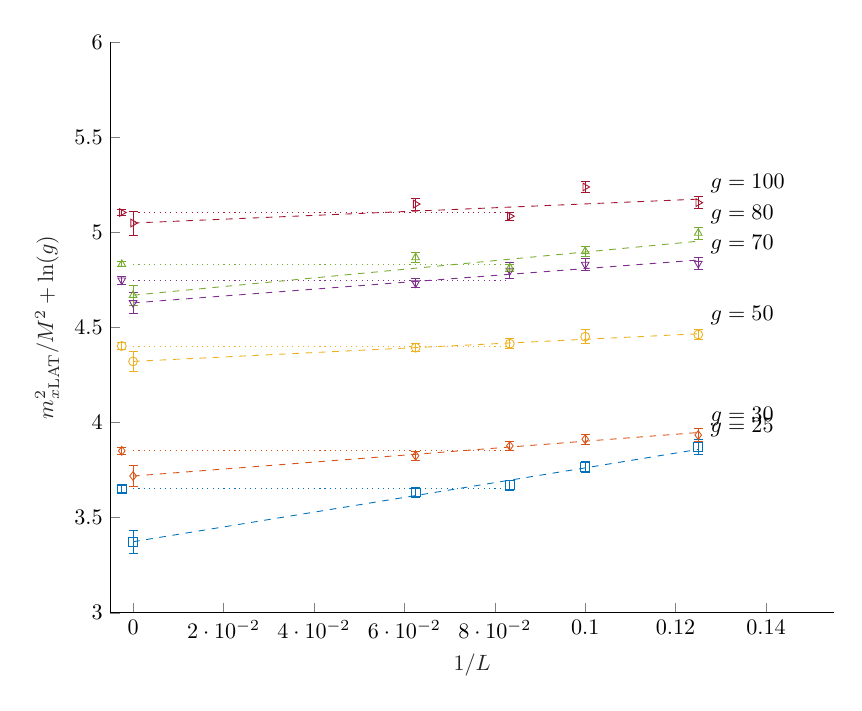
\begin{tikzpicture}[thick,scale=0.8, every node/.style={scale=1}]

\begin{axis}[%
width=4.521in,
height=3.566in,
at={(0.758in,0.481in)},
scale only axis,
xmin=-0.005,
xmax=0.155,
xlabel style={font=\color{white!15!black}},
xlabel={$1/L$},
ymin=3,
ymax=6,
ylabel style={font=\color{white!15!black}},
ylabel={$m_{x{\rm LAT}}^2/M^2 + \ln(g)$},
axis background/.style={fill=white},
axis x line*=bottom,
axis y line*=left
]
\addplot [color=mycolor1, dotted, forget plot]
  table[row sep=crcr]{%
0	3.65157214496374\\
0.00125	3.65157214496374\\
0.0025	3.65157214496374\\
0.00375	3.65157214496374\\
0.005	3.65157214496374\\
0.00625	3.65157214496374\\
0.0075	3.65157214496374\\
0.00875	3.65157214496374\\
0.01	3.65157214496374\\
0.01125	3.65157214496374\\
0.0125	3.65157214496374\\
0.01375	3.65157214496374\\
0.015	3.65157214496374\\
0.01625	3.65157214496374\\
0.0175	3.65157214496374\\
0.01875	3.65157214496374\\
0.02	3.65157214496374\\
0.02125	3.65157214496374\\
0.0225	3.65157214496374\\
0.02375	3.65157214496374\\
0.025	3.65157214496374\\
0.02625	3.65157214496374\\
0.0275	3.65157214496374\\
0.02875	3.65157214496374\\
0.03	3.65157214496374\\
0.03125	3.65157214496374\\
0.0325	3.65157214496374\\
0.03375	3.65157214496374\\
0.035	3.65157214496374\\
0.03625	3.65157214496374\\
0.0375	3.65157214496374\\
0.03875	3.65157214496374\\
0.04	3.65157214496374\\
0.04125	3.65157214496374\\
0.0425	3.65157214496374\\
0.04375	3.65157214496374\\
0.045	3.65157214496374\\
0.04625	3.65157214496374\\
0.0475	3.65157214496374\\
0.04875	3.65157214496374\\
0.05	3.65157214496374\\
0.05125	3.65157214496374\\
0.0525	3.65157214496374\\
0.05375	3.65157214496374\\
0.055	3.65157214496374\\
0.05625	3.65157214496374\\
0.0575	3.65157214496374\\
0.05875	3.65157214496374\\
0.06	3.65157214496374\\
0.06125	3.65157214496374\\
0.0625	3.65157214496374\\
0.06375	3.65157214496374\\
0.065	3.65157214496374\\
0.06625	3.65157214496374\\
0.0675	3.65157214496374\\
0.06875	3.65157214496374\\
0.07	3.65157214496374\\
0.07125	3.65157214496374\\
0.0725	3.65157214496374\\
0.07375	3.65157214496374\\
0.075	3.65157214496374\\
0.07625	3.65157214496374\\
0.0775	3.65157214496374\\
0.07875	3.65157214496374\\
0.08	3.65157214496374\\
0.08125	3.65157214496374\\
0.0825	3.65157214496374\\
};
\addplot [color=mycolor1, dashed, forget plot]
  table[row sep=crcr]{%
0	3.37349707235251\\
0.00125	3.37835025246733\\
0.0025	3.38320343258214\\
0.00375	3.38805661269696\\
0.005	3.39290979281177\\
0.00625	3.39776297292659\\
0.0075	3.4026161530414\\
0.00875	3.40746933315621\\
0.01	3.41232251327103\\
0.01125	3.41717569338584\\
0.0125	3.42202887350066\\
0.01375	3.42688205361547\\
0.015	3.43173523373029\\
0.01625	3.4365884138451\\
0.0175	3.44144159395991\\
0.01875	3.44629477407473\\
0.02	3.45114795418954\\
0.02125	3.45600113430436\\
0.0225	3.46085431441917\\
0.02375	3.46570749453398\\
0.025	3.4705606746488\\
0.02625	3.47541385476361\\
0.0275	3.48026703487843\\
0.02875	3.48512021499324\\
0.03	3.48997339510806\\
0.03125	3.49482657522287\\
0.0325	3.49967975533768\\
0.03375	3.5045329354525\\
0.035	3.50938611556731\\
0.03625	3.51423929568213\\
0.0375	3.51909247579694\\
0.03875	3.52394565591176\\
0.04	3.52879883602657\\
0.04125	3.53365201614138\\
0.0425	3.5385051962562\\
0.04375	3.54335837637101\\
0.045	3.54821155648583\\
0.04625	3.55306473660064\\
0.0475	3.55791791671546\\
0.04875	3.56277109683027\\
0.05	3.56762427694508\\
0.05125	3.5724774570599\\
0.0525	3.57733063717471\\
0.05375	3.58218381728953\\
0.055	3.58703699740434\\
0.05625	3.59189017751916\\
0.0575	3.59674335763397\\
0.05875	3.60159653774878\\
0.06	3.6064497178636\\
0.06125	3.61130289797841\\
0.0625	3.61615607809323\\
0.06375	3.62100925820804\\
0.065	3.62586243832286\\
0.06625	3.63071561843767\\
0.0675	3.63556879855248\\
0.06875	3.6404219786673\\
0.07	3.64527515878211\\
0.07125	3.65012833889693\\
0.0725	3.65498151901174\\
0.07375	3.65983469912656\\
0.075	3.66468787924137\\
0.07625	3.66954105935618\\
0.0775	3.674394239471\\
0.07875	3.67924741958581\\
0.08	3.68410059970063\\
0.08125	3.68895377981544\\
0.0825	3.69380695993026\\
0.08375	3.69866014004507\\
0.085	3.70351332015988\\
0.08625	3.7083665002747\\
0.0875	3.71321968038951\\
0.08875	3.71807286050433\\
0.09	3.72292604061914\\
0.09125	3.72777922073396\\
0.0925	3.73263240084877\\
0.09375	3.73748558096358\\
0.095	3.7423387610784\\
0.09625	3.74719194119321\\
0.0975	3.75204512130803\\
0.09875	3.75689830142284\\
0.1	3.76175148153765\\
0.10125	3.76660466165247\\
0.1025	3.77145784176728\\
0.10375	3.7763110218821\\
0.105	3.78116420199691\\
0.10625	3.78601738211173\\
0.1075	3.79087056222654\\
0.10875	3.79572374234135\\
0.11	3.80057692245617\\
0.11125	3.80543010257098\\
0.1125	3.8102832826858\\
0.11375	3.81513646280061\\
0.115	3.81998964291543\\
0.11625	3.82484282303024\\
0.1175	3.82969600314505\\
0.11875	3.83454918325987\\
0.12	3.83940236337468\\
0.12125	3.8442555434895\\
0.1225	3.84910872360431\\
0.12375	3.85396190371913\\
0.125	3.85881508383394\\
};
\addplot [color=mycolor1, draw=none, mark=square, mark options={solid, mycolor1}, forget plot]
 plot [error bars/.cd, y dir = both, y explicit]
 table[row sep=crcr, y error plus index=2, y error minus index=3]{%
0	3.37349707235251	0.0618188255511083	0.0618188255511083\\
-0.0025	3.65157214496374	0.0184735695510096	0.0184735695510096\\
0.125	3.87232330396237	0.0379326151867826	0.0379326151867826\\
0.1	3.76664431116438	0.0272639406130805	0.0272639406130805\\
0.0833333333333333	3.67001501590284	0.0259899619038176	0.0259899619038176\\
0.0625	3.63273926353459	0.0262633284740344	0.0262633284740344\\
};
\node[right, align=left]
at (axis cs:0.126,3.972) {$g = 25$};
\addplot [color=mycolor2, dotted, forget plot]
  table[row sep=crcr]{%
0	3.85138365745057\\
0.00125	3.85138365745057\\
0.0025	3.85138365745057\\
0.00375	3.85138365745057\\
0.005	3.85138365745057\\
0.00625	3.85138365745057\\
0.0075	3.85138365745057\\
0.00875	3.85138365745057\\
0.01	3.85138365745057\\
0.01125	3.85138365745057\\
0.0125	3.85138365745057\\
0.01375	3.85138365745057\\
0.015	3.85138365745057\\
0.01625	3.85138365745057\\
0.0175	3.85138365745057\\
0.01875	3.85138365745057\\
0.02	3.85138365745057\\
0.02125	3.85138365745057\\
0.0225	3.85138365745057\\
0.02375	3.85138365745057\\
0.025	3.85138365745057\\
0.02625	3.85138365745057\\
0.0275	3.85138365745057\\
0.02875	3.85138365745057\\
0.03	3.85138365745057\\
0.03125	3.85138365745057\\
0.0325	3.85138365745057\\
0.03375	3.85138365745057\\
0.035	3.85138365745057\\
0.03625	3.85138365745057\\
0.0375	3.85138365745057\\
0.03875	3.85138365745057\\
0.04	3.85138365745057\\
0.04125	3.85138365745057\\
0.0425	3.85138365745057\\
0.04375	3.85138365745057\\
0.045	3.85138365745057\\
0.04625	3.85138365745057\\
0.0475	3.85138365745057\\
0.04875	3.85138365745057\\
0.05	3.85138365745057\\
0.05125	3.85138365745057\\
0.0525	3.85138365745057\\
0.05375	3.85138365745057\\
0.055	3.85138365745057\\
0.05625	3.85138365745057\\
0.0575	3.85138365745057\\
0.05875	3.85138365745057\\
0.06	3.85138365745057\\
0.06125	3.85138365745057\\
0.0625	3.85138365745057\\
0.06375	3.85138365745057\\
0.065	3.85138365745057\\
0.06625	3.85138365745057\\
0.0675	3.85138365745057\\
0.06875	3.85138365745057\\
0.07	3.85138365745057\\
0.07125	3.85138365745057\\
0.0725	3.85138365745057\\
0.07375	3.85138365745057\\
0.075	3.85138365745057\\
0.07625	3.85138365745057\\
0.0775	3.85138365745057\\
0.07875	3.85138365745057\\
0.08	3.85138365745057\\
0.08125	3.85138365745057\\
0.0825	3.85138365745057\\
};
\addplot [color=mycolor2, dashed, forget plot]
  table[row sep=crcr]{%
0	3.71889969934731\\
0.00125	3.72118722048591\\
0.0025	3.7234747416245\\
0.00375	3.7257622627631\\
0.005	3.7280497839017\\
0.00625	3.7303373050403\\
0.0075	3.7326248261789\\
0.00875	3.73491234731749\\
0.01	3.73719986845609\\
0.01125	3.73948738959469\\
0.0125	3.74177491073329\\
0.01375	3.74406243187188\\
0.015	3.74634995301048\\
0.01625	3.74863747414908\\
0.0175	3.75092499528768\\
0.01875	3.75321251642627\\
0.02	3.75550003756487\\
0.02125	3.75778755870347\\
0.0225	3.76007507984207\\
0.02375	3.76236260098067\\
0.025	3.76465012211926\\
0.02625	3.76693764325786\\
0.0275	3.76922516439646\\
0.02875	3.77151268553506\\
0.03	3.77380020667365\\
0.03125	3.77608772781225\\
0.0325	3.77837524895085\\
0.03375	3.78066277008945\\
0.035	3.78295029122805\\
0.03625	3.78523781236664\\
0.0375	3.78752533350524\\
0.03875	3.78981285464384\\
0.04	3.79210037578244\\
0.04125	3.79438789692103\\
0.0425	3.79667541805963\\
0.04375	3.79896293919823\\
0.045	3.80125046033683\\
0.04625	3.80353798147543\\
0.0475	3.80582550261402\\
0.04875	3.80811302375262\\
0.05	3.81040054489122\\
0.05125	3.81268806602982\\
0.0525	3.81497558716841\\
0.05375	3.81726310830701\\
0.055	3.81955062944561\\
0.05625	3.82183815058421\\
0.0575	3.8241256717228\\
0.05875	3.8264131928614\\
0.06	3.828700714\\
0.06125	3.8309882351386\\
0.0625	3.8332757562772\\
0.06375	3.83556327741579\\
0.065	3.83785079855439\\
0.06625	3.84013831969299\\
0.0675	3.84242584083159\\
0.06875	3.84471336197018\\
0.07	3.84700088310878\\
0.07125	3.84928840424738\\
0.0725	3.85157592538598\\
0.07375	3.85386344652458\\
0.075	3.85615096766317\\
0.07625	3.85843848880177\\
0.0775	3.86072600994037\\
0.07875	3.86301353107897\\
0.08	3.86530105221756\\
0.08125	3.86758857335616\\
0.0825	3.86987609449476\\
0.08375	3.87216361563336\\
0.085	3.87445113677196\\
0.08625	3.87673865791055\\
0.0875	3.87902617904915\\
0.08875	3.88131370018775\\
0.09	3.88360122132635\\
0.09125	3.88588874246494\\
0.0925	3.88817626360354\\
0.09375	3.89046378474214\\
0.095	3.89275130588074\\
0.09625	3.89503882701934\\
0.0975	3.89732634815793\\
0.09875	3.89961386929653\\
0.1	3.90190139043513\\
0.10125	3.90418891157373\\
0.1025	3.90647643271232\\
0.10375	3.90876395385092\\
0.105	3.91105147498952\\
0.10625	3.91333899612812\\
0.1075	3.91562651726672\\
0.10875	3.91791403840531\\
0.11	3.92020155954391\\
0.11125	3.92248908068251\\
0.1125	3.92477660182111\\
0.11375	3.9270641229597\\
0.115	3.9293516440983\\
0.11625	3.9316391652369\\
0.1175	3.9339266863755\\
0.11875	3.93621420751409\\
0.12	3.93850172865269\\
0.12125	3.94078924979129\\
0.1225	3.94307677092989\\
0.12375	3.94536429206849\\
0.125	3.94765181320708\\
};
\addplot [color=mycolor2, draw=none, mark=diamond, mark options={solid, mycolor2}, forget plot]
 plot [error bars/.cd, y dir = both, y explicit]
 table[row sep=crcr, y error plus index=2, y error minus index=3]{%
0	3.71889969934731	0.056892614807216	0.056892614807216\\
-0.0025	3.85138365745057	0.0174330383037749	0.0174330383037749\\
0.125	3.93408185768866	0.0335523147449089	0.0335523147449089\\
0.1	3.91253199903651	0.0268764627738956	0.0268764627738956\\
0.0833333333333333	3.87732513623202	0.0247486927848557	0.0247486927848557\\
0.0625	3.82583528059023	0.0245604634118641	0.0245604634118641\\
};
\node[right, align=left]
at (axis cs:0.126,4.034) {$g = 30$};
\addplot [color=mycolor3, dotted, forget plot]
  table[row sep=crcr]{%
0	4.40261824194551\\
0.00125	4.40261824194551\\
0.0025	4.40261824194551\\
0.00375	4.40261824194551\\
0.005	4.40261824194551\\
0.00625	4.40261824194551\\
0.0075	4.40261824194551\\
0.00875	4.40261824194551\\
0.01	4.40261824194551\\
0.01125	4.40261824194551\\
0.0125	4.40261824194551\\
0.01375	4.40261824194551\\
0.015	4.40261824194551\\
0.01625	4.40261824194551\\
0.0175	4.40261824194551\\
0.01875	4.40261824194551\\
0.02	4.40261824194551\\
0.02125	4.40261824194551\\
0.0225	4.40261824194551\\
0.02375	4.40261824194551\\
0.025	4.40261824194551\\
0.02625	4.40261824194551\\
0.0275	4.40261824194551\\
0.02875	4.40261824194551\\
0.03	4.40261824194551\\
0.03125	4.40261824194551\\
0.0325	4.40261824194551\\
0.03375	4.40261824194551\\
0.035	4.40261824194551\\
0.03625	4.40261824194551\\
0.0375	4.40261824194551\\
0.03875	4.40261824194551\\
0.04	4.40261824194551\\
0.04125	4.40261824194551\\
0.0425	4.40261824194551\\
0.04375	4.40261824194551\\
0.045	4.40261824194551\\
0.04625	4.40261824194551\\
0.0475	4.40261824194551\\
0.04875	4.40261824194551\\
0.05	4.40261824194551\\
0.05125	4.40261824194551\\
0.0525	4.40261824194551\\
0.05375	4.40261824194551\\
0.055	4.40261824194551\\
0.05625	4.40261824194551\\
0.0575	4.40261824194551\\
0.05875	4.40261824194551\\
0.06	4.40261824194551\\
0.06125	4.40261824194551\\
0.0625	4.40261824194551\\
0.06375	4.40261824194551\\
0.065	4.40261824194551\\
0.06625	4.40261824194551\\
0.0675	4.40261824194551\\
0.06875	4.40261824194551\\
0.07	4.40261824194551\\
0.07125	4.40261824194551\\
0.0725	4.40261824194551\\
0.07375	4.40261824194551\\
0.075	4.40261824194551\\
0.07625	4.40261824194551\\
0.0775	4.40261824194551\\
0.07875	4.40261824194551\\
0.08	4.40261824194551\\
0.08125	4.40261824194551\\
0.0825	4.40261824194551\\
};
\addplot [color=mycolor3, dashed, forget plot]
  table[row sep=crcr]{%
0	4.32155158433652\\
0.00125	4.32300398305877\\
0.0025	4.32445638178101\\
0.00375	4.32590878050326\\
0.005	4.32736117922551\\
0.00625	4.32881357794775\\
0.0075	4.33026597667\\
0.00875	4.33171837539225\\
0.01	4.3331707741145\\
0.01125	4.33462317283674\\
0.0125	4.33607557155899\\
0.01375	4.33752797028124\\
0.015	4.33898036900348\\
0.01625	4.34043276772573\\
0.0175	4.34188516644798\\
0.01875	4.34333756517022\\
0.02	4.34478996389247\\
0.02125	4.34624236261472\\
0.0225	4.34769476133697\\
0.02375	4.34914716005921\\
0.025	4.35059955878146\\
0.02625	4.35205195750371\\
0.0275	4.35350435622595\\
0.02875	4.3549567549482\\
0.03	4.35640915367045\\
0.03125	4.35786155239269\\
0.0325	4.35931395111494\\
0.03375	4.36076634983719\\
0.035	4.36221874855944\\
0.03625	4.36367114728168\\
0.0375	4.36512354600393\\
0.03875	4.36657594472618\\
0.04	4.36802834344842\\
0.04125	4.36948074217067\\
0.0425	4.37093314089292\\
0.04375	4.37238553961516\\
0.045	4.37383793833741\\
0.04625	4.37529033705966\\
0.0475	4.3767427357819\\
0.04875	4.37819513450415\\
0.05	4.3796475332264\\
0.05125	4.38109993194865\\
0.0525	4.38255233067089\\
0.05375	4.38400472939314\\
0.055	4.38545712811539\\
0.05625	4.38690952683763\\
0.0575	4.38836192555988\\
0.05875	4.38981432428213\\
0.06	4.39126672300438\\
0.06125	4.39271912172662\\
0.0625	4.39417152044887\\
0.06375	4.39562391917112\\
0.065	4.39707631789336\\
0.06625	4.39852871661561\\
0.0675	4.39998111533786\\
0.06875	4.4014335140601\\
0.07	4.40288591278235\\
0.07125	4.4043383115046\\
0.0725	4.40579071022684\\
0.07375	4.40724310894909\\
0.075	4.40869550767134\\
0.07625	4.41014790639359\\
0.0775	4.41160030511583\\
0.07875	4.41305270383808\\
0.08	4.41450510256033\\
0.08125	4.41595750128257\\
0.0825	4.41740990000482\\
0.08375	4.41886229872707\\
0.085	4.42031469744931\\
0.08625	4.42176709617156\\
0.0875	4.42321949489381\\
0.08875	4.42467189361606\\
0.09	4.4261242923383\\
0.09125	4.42757669106055\\
0.0925	4.4290290897828\\
0.09375	4.43048148850504\\
0.095	4.43193388722729\\
0.09625	4.43338628594954\\
0.0975	4.43483868467179\\
0.09875	4.43629108339403\\
0.1	4.43774348211628\\
0.10125	4.43919588083853\\
0.1025	4.44064827956077\\
0.10375	4.44210067828302\\
0.105	4.44355307700527\\
0.10625	4.44500547572751\\
0.1075	4.44645787444976\\
0.10875	4.44791027317201\\
0.11	4.44936267189425\\
0.11125	4.4508150706165\\
0.1125	4.45226746933875\\
0.11375	4.453719868061\\
0.115	4.45517226678324\\
0.11625	4.45662466550549\\
0.1175	4.45807706422774\\
0.11875	4.45952946294998\\
0.12	4.46098186167223\\
0.12125	4.46243426039448\\
0.1225	4.46388665911672\\
0.12375	4.46533905783897\\
0.125	4.46679145656122\\
};
\addplot [color=mycolor3, draw=none, mark=o, mark options={solid, mycolor3}, forget plot]
 plot [error bars/.cd, y dir = both, y explicit]
 table[row sep=crcr, y error plus index=2, y error minus index=3]{%
0	4.32155158433652	0.0509813301288695	0.0509813301288695\\
-0.0025	4.40261824194551	0.0170372725948838	0.0170372725948838\\
0.125	4.46301393463463	0.0278598622105965	0.0278598622105965\\
0.1	4.4517019716889	0.0353815860464713	0.0353815860464713\\
0.0833333333333333	4.41463608534354	0.0261559054897396	0.0261559054897396\\
0.0625	4.3937613408905	0.0224541896115678	0.0224541896115678\\
};
\node[right, align=left]
at (axis cs:0.126,4.563) {$g = 50$};
\addplot [color=mycolor4, dotted, forget plot]
  table[row sep=crcr]{%
0	4.74858255781121\\
0.00125	4.74858255781121\\
0.0025	4.74858255781121\\
0.00375	4.74858255781121\\
0.005	4.74858255781121\\
0.00625	4.74858255781121\\
0.0075	4.74858255781121\\
0.00875	4.74858255781121\\
0.01	4.74858255781121\\
0.01125	4.74858255781121\\
0.0125	4.74858255781121\\
0.01375	4.74858255781121\\
0.015	4.74858255781121\\
0.01625	4.74858255781121\\
0.0175	4.74858255781121\\
0.01875	4.74858255781121\\
0.02	4.74858255781121\\
0.02125	4.74858255781121\\
0.0225	4.74858255781121\\
0.02375	4.74858255781121\\
0.025	4.74858255781121\\
0.02625	4.74858255781121\\
0.0275	4.74858255781121\\
0.02875	4.74858255781121\\
0.03	4.74858255781121\\
0.03125	4.74858255781121\\
0.0325	4.74858255781121\\
0.03375	4.74858255781121\\
0.035	4.74858255781121\\
0.03625	4.74858255781121\\
0.0375	4.74858255781121\\
0.03875	4.74858255781121\\
0.04	4.74858255781121\\
0.04125	4.74858255781121\\
0.0425	4.74858255781121\\
0.04375	4.74858255781121\\
0.045	4.74858255781121\\
0.04625	4.74858255781121\\
0.0475	4.74858255781121\\
0.04875	4.74858255781121\\
0.05	4.74858255781121\\
0.05125	4.74858255781121\\
0.0525	4.74858255781121\\
0.05375	4.74858255781121\\
0.055	4.74858255781121\\
0.05625	4.74858255781121\\
0.0575	4.74858255781121\\
0.05875	4.74858255781121\\
0.06	4.74858255781121\\
0.06125	4.74858255781121\\
0.0625	4.74858255781121\\
0.06375	4.74858255781121\\
0.065	4.74858255781121\\
0.06625	4.74858255781121\\
0.0675	4.74858255781121\\
0.06875	4.74858255781121\\
0.07	4.74858255781121\\
0.07125	4.74858255781121\\
0.0725	4.74858255781121\\
0.07375	4.74858255781121\\
0.075	4.74858255781121\\
0.07625	4.74858255781121\\
0.0775	4.74858255781121\\
0.07875	4.74858255781121\\
0.08	4.74858255781121\\
0.08125	4.74858255781121\\
0.0825	4.74858255781121\\
};
\addplot [color=mycolor4, dashed, forget plot]
  table[row sep=crcr]{%
0	4.62934195767659\\
0.00125	4.63159426871648\\
0.0025	4.63384657975636\\
0.00375	4.63609889079625\\
0.005	4.63835120183613\\
0.00625	4.64060351287602\\
0.0075	4.6428558239159\\
0.00875	4.64510813495579\\
0.01	4.64736044599567\\
0.01125	4.64961275703556\\
0.0125	4.65186506807545\\
0.01375	4.65411737911533\\
0.015	4.65636969015522\\
0.01625	4.6586220011951\\
0.0175	4.66087431223499\\
0.01875	4.66312662327487\\
0.02	4.66537893431476\\
0.02125	4.66763124535465\\
0.0225	4.66988355639453\\
0.02375	4.67213586743442\\
0.025	4.6743881784743\\
0.02625	4.67664048951419\\
0.0275	4.67889280055407\\
0.02875	4.68114511159396\\
0.03	4.68339742263384\\
0.03125	4.68564973367373\\
0.0325	4.68790204471361\\
0.03375	4.6901543557535\\
0.035	4.69240666679339\\
0.03625	4.69465897783327\\
0.0375	4.69691128887316\\
0.03875	4.69916359991304\\
0.04	4.70141591095293\\
0.04125	4.70366822199281\\
0.0425	4.7059205330327\\
0.04375	4.70817284407258\\
0.045	4.71042515511247\\
0.04625	4.71267746615236\\
0.0475	4.71492977719224\\
0.04875	4.71718208823213\\
0.05	4.71943439927201\\
0.05125	4.7216867103119\\
0.0525	4.72393902135178\\
0.05375	4.72619133239167\\
0.055	4.72844364343155\\
0.05625	4.73069595447144\\
0.0575	4.73294826551133\\
0.05875	4.73520057655121\\
0.06	4.7374528875911\\
0.06125	4.73970519863098\\
0.0625	4.74195750967087\\
0.06375	4.74420982071075\\
0.065	4.74646213175064\\
0.06625	4.74871444279052\\
0.0675	4.75096675383041\\
0.06875	4.75321906487029\\
0.07	4.75547137591018\\
0.07125	4.75772368695007\\
0.0725	4.75997599798995\\
0.07375	4.76222830902984\\
0.075	4.76448062006972\\
0.07625	4.76673293110961\\
0.0775	4.76898524214949\\
0.07875	4.77123755318938\\
0.08	4.77348986422926\\
0.08125	4.77574217526915\\
0.0825	4.77799448630904\\
0.08375	4.78024679734892\\
0.085	4.78249910838881\\
0.08625	4.78475141942869\\
0.0875	4.78700373046858\\
0.08875	4.78925604150846\\
0.09	4.79150835254835\\
0.09125	4.79376066358823\\
0.0925	4.79601297462812\\
0.09375	4.79826528566801\\
0.095	4.80051759670789\\
0.09625	4.80276990774778\\
0.0975	4.80502221878766\\
0.09875	4.80727452982755\\
0.1	4.80952684086743\\
0.10125	4.81177915190732\\
0.1025	4.8140314629472\\
0.10375	4.81628377398709\\
0.105	4.81853608502697\\
0.10625	4.82078839606686\\
0.1075	4.82304070710675\\
0.10875	4.82529301814663\\
0.11	4.82754532918652\\
0.11125	4.8297976402264\\
0.1125	4.83204995126629\\
0.11375	4.83430226230617\\
0.115	4.83655457334606\\
0.11625	4.83880688438594\\
0.1175	4.84105919542583\\
0.11875	4.84331150646572\\
0.12	4.8455638175056\\
0.12125	4.84781612854549\\
0.1225	4.85006843958537\\
0.12375	4.85232075062526\\
0.125	4.85457306166514\\
};
\addplot [color=mycolor4, draw=none, mark=triangle, mark options={solid, rotate=180, mycolor4}, forget plot]
 plot [error bars/.cd, y dir = both, y explicit]
 table[row sep=crcr, y error plus index=2, y error minus index=3]{%
0	4.62934195767659	0.0554586752863889	0.0554586752863889\\
-0.0025	4.74858255781121	0.0201789301099058	0.0201789301099058\\
0.125	4.83608416461684	0.0326667253608137	0.0326667253608137\\
0.1	4.8314925380709	0.0312599063930023	0.0312599063930023\\
0.0833333333333333	4.79967636407131	0.0418601604554231	0.0418601604554231\\
0.0625	4.73311523381499	0.023031612852148	0.023031612852148\\
};
\node[right, align=left]
at (axis cs:0.126,4.936) {$g = 70$};
\addplot [color=mycolor5, dotted, forget plot]
  table[row sep=crcr]{%
0	4.83258842102378\\
0.00125	4.83258842102378\\
0.0025	4.83258842102378\\
0.00375	4.83258842102378\\
0.005	4.83258842102378\\
0.00625	4.83258842102378\\
0.0075	4.83258842102378\\
0.00875	4.83258842102378\\
0.01	4.83258842102378\\
0.01125	4.83258842102378\\
0.0125	4.83258842102378\\
0.01375	4.83258842102378\\
0.015	4.83258842102378\\
0.01625	4.83258842102378\\
0.0175	4.83258842102378\\
0.01875	4.83258842102378\\
0.02	4.83258842102378\\
0.02125	4.83258842102378\\
0.0225	4.83258842102378\\
0.02375	4.83258842102378\\
0.025	4.83258842102378\\
0.02625	4.83258842102378\\
0.0275	4.83258842102378\\
0.02875	4.83258842102378\\
0.03	4.83258842102378\\
0.03125	4.83258842102378\\
0.0325	4.83258842102378\\
0.03375	4.83258842102378\\
0.035	4.83258842102378\\
0.03625	4.83258842102378\\
0.0375	4.83258842102378\\
0.03875	4.83258842102378\\
0.04	4.83258842102378\\
0.04125	4.83258842102378\\
0.0425	4.83258842102378\\
0.04375	4.83258842102378\\
0.045	4.83258842102378\\
0.04625	4.83258842102378\\
0.0475	4.83258842102378\\
0.04875	4.83258842102378\\
0.05	4.83258842102378\\
0.05125	4.83258842102378\\
0.0525	4.83258842102378\\
0.05375	4.83258842102378\\
0.055	4.83258842102378\\
0.05625	4.83258842102378\\
0.0575	4.83258842102378\\
0.05875	4.83258842102378\\
0.06	4.83258842102378\\
0.06125	4.83258842102378\\
0.0625	4.83258842102378\\
0.06375	4.83258842102378\\
0.065	4.83258842102378\\
0.06625	4.83258842102378\\
0.0675	4.83258842102378\\
0.06875	4.83258842102378\\
0.07	4.83258842102378\\
0.07125	4.83258842102378\\
0.0725	4.83258842102378\\
0.07375	4.83258842102378\\
0.075	4.83258842102378\\
0.07625	4.83258842102378\\
0.0775	4.83258842102378\\
0.07875	4.83258842102378\\
0.08	4.83258842102378\\
0.08125	4.83258842102378\\
0.0825	4.83258842102378\\
};
\addplot [color=mycolor5, dashed, forget plot]
  table[row sep=crcr]{%
0	4.6697227903436\\
0.00125	4.67256142977422\\
0.0025	4.67540006920484\\
0.00375	4.67823870863545\\
0.005	4.68107734806607\\
0.00625	4.68391598749669\\
0.0075	4.6867546269273\\
0.00875	4.68959326635792\\
0.01	4.69243190578854\\
0.01125	4.69527054521915\\
0.0125	4.69810918464977\\
0.01375	4.70094782408039\\
0.015	4.70378646351101\\
0.01625	4.70662510294162\\
0.0175	4.70946374237224\\
0.01875	4.71230238180286\\
0.02	4.71514102123347\\
0.02125	4.71797966066409\\
0.0225	4.72081830009471\\
0.02375	4.72365693952533\\
0.025	4.72649557895594\\
0.02625	4.72933421838656\\
0.0275	4.73217285781718\\
0.02875	4.7350114972478\\
0.03	4.73785013667841\\
0.03125	4.74068877610903\\
0.0325	4.74352741553965\\
0.03375	4.74636605497026\\
0.035	4.74920469440088\\
0.03625	4.7520433338315\\
0.0375	4.75488197326212\\
0.03875	4.75772061269273\\
0.04	4.76055925212335\\
0.04125	4.76339789155397\\
0.0425	4.76623653098458\\
0.04375	4.7690751704152\\
0.045	4.77191380984582\\
0.04625	4.77475244927644\\
0.0475	4.77759108870705\\
0.04875	4.78042972813767\\
0.05	4.78326836756829\\
0.05125	4.7861070069989\\
0.0525	4.78894564642952\\
0.05375	4.79178428586014\\
0.055	4.79462292529075\\
0.05625	4.79746156472137\\
0.0575	4.80030020415199\\
0.05875	4.80313884358261\\
0.06	4.80597748301322\\
0.06125	4.80881612244384\\
0.0625	4.81165476187446\\
0.06375	4.81449340130508\\
0.065	4.81733204073569\\
0.06625	4.82017068016631\\
0.0675	4.82300931959693\\
0.06875	4.82584795902754\\
0.07	4.82868659845816\\
0.07125	4.83152523788878\\
0.0725	4.83436387731939\\
0.07375	4.83720251675001\\
0.075	4.84004115618063\\
0.07625	4.84287979561125\\
0.0775	4.84571843504186\\
0.07875	4.84855707447248\\
0.08	4.8513957139031\\
0.08125	4.85423435333372\\
0.0825	4.85707299276433\\
0.08375	4.85991163219495\\
0.085	4.86275027162557\\
0.08625	4.86558891105618\\
0.0875	4.8684275504868\\
0.08875	4.87126618991742\\
0.09	4.87410482934803\\
0.09125	4.87694346877865\\
0.0925	4.87978210820927\\
0.09375	4.88262074763989\\
0.095	4.8854593870705\\
0.09625	4.88829802650112\\
0.0975	4.89113666593174\\
0.09875	4.89397530536236\\
0.1	4.89681394479297\\
0.10125	4.89965258422359\\
0.1025	4.90249122365421\\
0.10375	4.90532986308482\\
0.105	4.90816850251544\\
0.10625	4.91100714194606\\
0.1075	4.91384578137667\\
0.10875	4.91668442080729\\
0.11	4.91952306023791\\
0.11125	4.92236169966853\\
0.1125	4.92520033909914\\
0.11375	4.92803897852976\\
0.115	4.93087761796038\\
0.11625	4.933716257391\\
0.1175	4.93655489682161\\
0.11875	4.93939353625223\\
0.12	4.94223217568285\\
0.12125	4.94507081511346\\
0.1225	4.94790945454408\\
0.12375	4.9507480939747\\
0.125	4.95358673340531\\
};
\addplot [color=mycolor5, draw=none, mark=triangle, mark options={solid, mycolor5}, forget plot]
 plot [error bars/.cd, y dir = both, y explicit]
 table[row sep=crcr, y error plus index=2, y error minus index=3]{%
0	4.6697227903436	0.0537296626042618	0.0537296626042618\\
-0.0025	4.83258842102378	0.0143086619540424	0.0143086619540424\\
0.125	4.99627931425365	0.03090870882112	0.03090870882112\\
0.1	4.90018761470393	0.0253271768707453	0.0253271768707453\\
0.0833333333333333	4.81434766210215	0.0176311840538604	0.0176311840538604\\
0.0625	4.86778012162998	0.0244895133180309	0.0244895133180309\\
};
\node[right, align=left]
at (axis cs:0.126,5.096) {$g = 80$};
\addplot [color=mycolor6, dotted, forget plot]
  table[row sep=crcr]{%
0	5.10449279477131\\
0.00125	5.10449279477131\\
0.0025	5.10449279477131\\
0.00375	5.10449279477131\\
0.005	5.10449279477131\\
0.00625	5.10449279477131\\
0.0075	5.10449279477131\\
0.00875	5.10449279477131\\
0.01	5.10449279477131\\
0.01125	5.10449279477131\\
0.0125	5.10449279477131\\
0.01375	5.10449279477131\\
0.015	5.10449279477131\\
0.01625	5.10449279477131\\
0.0175	5.10449279477131\\
0.01875	5.10449279477131\\
0.02	5.10449279477131\\
0.02125	5.10449279477131\\
0.0225	5.10449279477131\\
0.02375	5.10449279477131\\
0.025	5.10449279477131\\
0.02625	5.10449279477131\\
0.0275	5.10449279477131\\
0.02875	5.10449279477131\\
0.03	5.10449279477131\\
0.03125	5.10449279477131\\
0.0325	5.10449279477131\\
0.03375	5.10449279477131\\
0.035	5.10449279477131\\
0.03625	5.10449279477131\\
0.0375	5.10449279477131\\
0.03875	5.10449279477131\\
0.04	5.10449279477131\\
0.04125	5.10449279477131\\
0.0425	5.10449279477131\\
0.04375	5.10449279477131\\
0.045	5.10449279477131\\
0.04625	5.10449279477131\\
0.0475	5.10449279477131\\
0.04875	5.10449279477131\\
0.05	5.10449279477131\\
0.05125	5.10449279477131\\
0.0525	5.10449279477131\\
0.05375	5.10449279477131\\
0.055	5.10449279477131\\
0.05625	5.10449279477131\\
0.0575	5.10449279477131\\
0.05875	5.10449279477131\\
0.06	5.10449279477131\\
0.06125	5.10449279477131\\
0.0625	5.10449279477131\\
0.06375	5.10449279477131\\
0.065	5.10449279477131\\
0.06625	5.10449279477131\\
0.0675	5.10449279477131\\
0.06875	5.10449279477131\\
0.07	5.10449279477131\\
0.07125	5.10449279477131\\
0.0725	5.10449279477131\\
0.07375	5.10449279477131\\
0.075	5.10449279477131\\
0.07625	5.10449279477131\\
0.0775	5.10449279477131\\
0.07875	5.10449279477131\\
0.08	5.10449279477131\\
0.08125	5.10449279477131\\
0.0825	5.10449279477131\\
};
\addplot [color=mycolor6, dashed, forget plot]
  table[row sep=crcr]{%
0	5.04912189037121\\
0.00125	5.05037791691835\\
0.0025	5.0516339434655\\
0.00375	5.05288997001264\\
0.005	5.05414599655978\\
0.00625	5.05540202310692\\
0.0075	5.05665804965407\\
0.00875	5.05791407620121\\
0.01	5.05917010274835\\
0.01125	5.0604261292955\\
0.0125	5.06168215584264\\
0.01375	5.06293818238978\\
0.015	5.06419420893692\\
0.01625	5.06545023548407\\
0.0175	5.06670626203121\\
0.01875	5.06796228857835\\
0.02	5.06921831512549\\
0.02125	5.07047434167264\\
0.0225	5.07173036821978\\
0.02375	5.07298639476692\\
0.025	5.07424242131407\\
0.02625	5.07549844786121\\
0.0275	5.07675447440835\\
0.02875	5.07801050095549\\
0.03	5.07926652750264\\
0.03125	5.08052255404978\\
0.0325	5.08177858059692\\
0.03375	5.08303460714406\\
0.035	5.08429063369121\\
0.03625	5.08554666023835\\
0.0375	5.08680268678549\\
0.03875	5.08805871333264\\
0.04	5.08931473987978\\
0.04125	5.09057076642692\\
0.0425	5.09182679297406\\
0.04375	5.09308281952121\\
0.045	5.09433884606835\\
0.04625	5.09559487261549\\
0.0475	5.09685089916263\\
0.04875	5.09810692570978\\
0.05	5.09936295225692\\
0.05125	5.10061897880406\\
0.0525	5.10187500535121\\
0.05375	5.10313103189835\\
0.055	5.10438705844549\\
0.05625	5.10564308499263\\
0.0575	5.10689911153978\\
0.05875	5.10815513808692\\
0.06	5.10941116463406\\
0.06125	5.11066719118121\\
0.0625	5.11192321772835\\
0.06375	5.11317924427549\\
0.065	5.11443527082263\\
0.06625	5.11569129736978\\
0.0675	5.11694732391692\\
0.06875	5.11820335046406\\
0.07	5.1194593770112\\
0.07125	5.12071540355835\\
0.0725	5.12197143010549\\
0.07375	5.12322745665263\\
0.075	5.12448348319977\\
0.07625	5.12573950974692\\
0.0775	5.12699553629406\\
0.07875	5.1282515628412\\
0.08	5.12950758938835\\
0.08125	5.13076361593549\\
0.0825	5.13201964248263\\
0.08375	5.13327566902977\\
0.085	5.13453169557692\\
0.08625	5.13578772212406\\
0.0875	5.1370437486712\\
0.08875	5.13829977521834\\
0.09	5.13955580176549\\
0.09125	5.14081182831263\\
0.0925	5.14206785485977\\
0.09375	5.14332388140692\\
0.095	5.14457990795406\\
0.09625	5.1458359345012\\
0.0975	5.14709196104834\\
0.09875	5.14834798759549\\
0.1	5.14960401414263\\
0.10125	5.15086004068977\\
0.1025	5.15211606723692\\
0.10375	5.15337209378406\\
0.105	5.1546281203312\\
0.10625	5.15588414687834\\
0.1075	5.15714017342549\\
0.10875	5.15839619997263\\
0.11	5.15965222651977\\
0.11125	5.16090825306691\\
0.1125	5.16216427961406\\
0.11375	5.1634203061612\\
0.115	5.16467633270834\\
0.11625	5.16593235925549\\
0.1175	5.16718838580263\\
0.11875	5.16844441234977\\
0.12	5.16970043889691\\
0.12125	5.17095646544406\\
0.1225	5.1722124919912\\
0.12375	5.17346851853834\\
0.125	5.17472454508548\\
};
\addplot [color=mycolor6, draw=none, mark=triangle, mark options={solid, rotate=270, mycolor6}, forget plot]
 plot [error bars/.cd, y dir = both, y explicit]
 table[row sep=crcr, y error plus index=2, y error minus index=3]{%
0	5.04912189037121	0.0630194705105146	0.0630194705105146\\
-0.0025	5.10449279477131	0.0173236358422466	0.0173236358422466\\
0.125	5.15619365631232	0.0322590633641977	0.0322590633641977\\
0.1	5.23859166537553	0.031240582639804	0.031240582639804\\
0.0833333333333333	5.0851864892318	0.0207516032841688	0.0207516032841688\\
0.0625	5.14888410246905	0.0314666883013627	0.0314666883013627\\
};
\node[right, align=left]
at (axis cs:0.126,5.256) {$g = 100$};
\end{axis}
\end{tikzpicture}%
\caption{Plot of $m_{x\rm LAT}^{2}(L,g)/M^{2}= m_{x}^{2}(g)/m^{2}+\mathcal{O}(1/L)$ for $LM=4$ and $r=0$, as from fits to connected correlators discussed in section \ref{sec: xx_corr}. To ensure better visibility of the fits at different $g$ values, $\ln g$ has been added. Dashed lines represent a linear fit to all the data points for one value of $g$, while for dotted lines the fit is to a constant and only contains the two smallest lattice spacings. Multiple points at the same value of $g$ and $L$ indicate multiple replica.
\label{fig: mx_r0_cont_lim}}
\end{figure}
%
%
%
\begin{figure}
\centering
\input{Plots/mx_vs_g_r0_2}
\caption{Continuum extrapolation for the $x$ field mass as a function of the bare continuum coupling $g_{\rm c}=0.04\,g$ with data points obtained from simulations without a \names{Wilson} term. Data points are obtained as continuum extrapolations from the linear fits in \autoref{fig: mx_r0_cont_lim}. The dotted line indicates the perturbative prediction according to (\ref{eq: m_x}).
\label{fig: mx_vs_g_r0}}
\end{figure}
%
%
%
\begin{figure}
\centering
\input{Plots/mx_vs_g_r0}
\caption{Continuum extrapolation for the $x$ field mass as a function of the bare continuum coupling $g_{\rm c}=0.04\,g$ with data points obtained from simulations without a \names{Wilson} term. Data points are obtained as fits to a constant from the two finest lattices where cutoff effects are assumed to be neglectable. The dotted line indicates the perturbative prediction according to (\ref{eq: m_x}).
\label{fig: mx_vs_g_r0_plateau}}
\end{figure}
%
%
%
\subsection*{Pfaffian sign}
Throughout the investigations of the properties of the fermion matrix in section \ref{sec: matrix_prop} we found that the \names{Pfaffian} can only change its sign if purely real or imaginary eigenvalues transit through zero. So if we start from a configuration with positive \names{Pfaffian} and ensure a sufficiently large separation of the smallest eigenvalues from zero, then the \names{Pfaffian} will remain positive and hence acts as a valid probability density for the RHMC. For a representative amount of configurations we analyse the spectrum of the operator $\hat{\mathcal{O}}_{\rm F}\hat{\mathcal{O}}_{\rm F}^{\dagger}$ (which has eigenvalues $\vert \lambda_{i}\vert^{2}$, whereas $\lambda_{i}$ are eigenvalues of $\hat{\mathcal{O}}_{\rm F}$) and extract the smallest eigenvalues. Their distribution is shown in \autoref{fig: ev_dist} on the left for $L=12$ and $g=5,10,30$. For $g=10,30$ we plot the mean of such distributions divided by their standard deviation for different values of $L$ in \autoref{fig: ev_zero_gap}. This illustrates the separation from zero in units of standard deviations and we observe such a separation by at least 3 standard deviations which (if we assume the distribution in \autoref{fig: ev_dist} to be \names{Gaussian}) makes it very unlikely for any eigenvalue to get to close to zero for $g\geq 10$. For finer lattice spacings this separation tends to increase and we thus do not expect any problems in taking the continuum limit. This eliminates sign problems for the regime of $g\geq 10$. For $g=5$ we basically introduce a lower bound for the eigenvalues with the twisted mass term in the reweighting and if this is adjusted to be high enough then this method should be sufficient to ensure a positive \names{Pfaffian}. Nonetheless it would be good practice to find a method to check for sign flips also during simulations.
%
%
%
\begin{figure}
\centering
% This file was created by matlab2tikz.
%
%The latest updates can be retrieved from
%  http://www.mathworks.com/matlabcentral/fileexchange/22022-matlab2tikz-matlab2tikz
%where you can also make suggestions and rate matlab2tikz.
%
\begin{tikzpicture}[thick,scale=0.8, every node/.style={scale=1}]

\begin{axis}[%
width=4.521in,
height=3.566in,
at={(0.758in,0.481in)},
scale only axis,
xmin=0,
xmax=0.13,
xtick={0,0.041666666666666664,0.0625,0.08333333333333333,0.1,0.125},
xticklabels={{0},{1/24},{1/16},{1/12},{1/10},{1/8}},
xlabel style={font=\color{white!15!black}},
xlabel={$1/L$},
ymin=0,
ymax=14,
ylabel style={font=\color{white!15!black}},
ylabel={$\langle \lambda_{\rm min}\rangle/\sigma_{\rm min}$},
axis background/.style={fill=white},
axis x line*=bottom,
axis y line*=left,
legend style={legend cell align=left, align=left, draw=white!15!black}
]
\addplot [color=blue, draw=none, mark=+, mark options={solid, blue}]
 plot [error bars/.cd, y dir = both, y explicit]
 table[row sep=crcr, y error plus index=2, y error minus index=3]{%
0.125	8.62082875751349	1.40837219358935	1.40837219358935\\
0.1	8.41913345231103	1.32250879479266	1.32250879479266\\
0.0833333333333333	8.6120262021668	0.874072829704015	0.874072829704015\\
0.0625	10.1236640025576	2.24580483798358	2.24580483798358\\
};
\addlegendentry{$g = 30$}

\addplot [color=black, draw=none, mark=o, mark options={solid, black}]
 plot [error bars/.cd, y dir = both, y explicit]
 table[row sep=crcr, y error plus index=2, y error minus index=3]{%
0.125	3.18915709275261	0.335168492707627	0.335168492707627\\
0.1	3.65390487842978	0.745923013957024	0.745923013957024\\
0.0833333333333333	3.20158297890721	0.228736283611952	0.228736283611952\\
0.0625	4.51214838498055	0.339023282750031	0.339023282750031\\
0.0416666666666667	4.5353861107916	0.777440619874027	0.777440619874027\\
};
\addlegendentry{$g = 10$}

\end{axis}
\end{tikzpicture}%
\caption{In \autoref{fig: ev_dist} on the left we saw the distribution of the minimal eigenvalues of $\hat{\mathcal{O}}_{\rm F}\hat{\mathcal{O}}_{\rm F}^{\dagger}$ for $L=12$ and multiple $g$. Here we plot mean over standard deviation of such distributions for $g=10,30$ and several values of $L$. Every point was derived from the minimal eigenvalues of 400 configurations.
\label{fig: ev_zero_gap}}
\end{figure}